\documentclass[english,t]{beamer}
%\documentclass[handout,english]{beamer}

\usepackage[T1]{fontenc}
\usepackage[utf8]{inputenc}
\usepackage{newtxtext} % times
%\usepackage[scaled=.95]{cabin} % sans serif
\usepackage{amsmath}
\usepackage[varqu,varl]{inconsolata} % typewriter
\usepackage[varg]{newtxmath}
\usefonttheme[onlymath]{serif} % beamer font theme
\usepackage{microtype}
\usepackage{afterpage}
\usepackage{url}
\urlstyle{same}
%\usepackage{amsbsy}
%\usepackage{eucal}
\usepackage{rotating}
%\usepackage{bm}
\usepackage{pdfpages}
\usepackage{algorithm}
\usepackage[noend]{algpseudocode}
\usepackage{booktabs}
\usepackage{listings}
\usepackage{lstbayes}
\graphicspath{{/home/ave/doc/images/}{}{../teranaloppu/}{../metodi/}{../slides/Hartikainen/}{../gphealth/}{../2008_09_RSS2008/}{../gphealth/}{../jyvaskyla2009/}{../nbbc2009/}{../gphealth/hippics/}{../euroheis2010/}{../pubgensens2011/}{../reykjavik2013/}{../liverpool2013/}{../../gpstuff/doc/}{./images/}{../aalto_stochastic/}{figs/}{../Stancon2018Helsinki/figs/}{../../paper/cvapprox/}{../gppa2017/}{../valencia2017/}{../../paper/combine_predictive_distribution/tex/}{../venice2018/figs/}{./figs/}}

% minted
\usepackage{minted}
\setminted{highlightcolor=yellow!25}
\newmintinline{r}{}
% The following is adjusted from
% https://tex.stackexchange.com/questions/548592/changing-all-colors-to-black-white-using-minted-sty
\makeatletter
\newcommand{\minted@style@bw}{%
  \renewcommand\fcolorbox[3][]{##3}%
  \renewcommand\textcolor[3][]{##3}%
  \color{gray}
}
% define new minted option "gray"
\minted@def@opt@switch{gray}
\fvset{formatcom*={%
  \ifthenelse{\equal{\minted@get@opt{gray}{true}}{true}}
  {\minted@style@bw}{}%
}}
\makeatother
% The following is ajusted from
% https://tex.stackexchange.com/questions/74459/remove-space-before-colorbox
\newcommand{\reducedstrut}{\vrule width 0pt height .9\ht\strutbox depth .9\dp\strutbox\relax}
\newcommand{\highlight}[1]{%
  \begingroup
  \setlength{\fboxsep}{0pt}%  
  \colorbox{yellow!30}{\reducedstrut\detokenize{#1}\/}%
  \endgroup
}

\usepackage{natbib}
\bibliographystyle{apalike}

\mode<presentation>
{
  \setbeamercovered{invisible}
  \setbeamertemplate{itemize items}[circle]
  \setbeamercolor{frametitle}{bg=white,fg=navyblue}
  \setbeamertemplate{navigation symbols}{}
  \setbeamertemplate{headline}[default]{}
  \setbeamertemplate{footline}[split]
  % \setbeamertemplate{headline}[text line]{\insertsection}
  \setbeamertemplate{footline}[frame number]
}

\pdfinfo{            
  /Title      (BDA, Lecture 9) 
  /Author     (Aki Vehtari) % 
  /Keywords   (Bayesian data analysis)
}

%%%%%%%%%%%%%%%%%%% for tikz figures %%%%%%%%%%%%%%%%%%%%%%%%%%
\usepackage{ifthen}
\usepackage{tikz,pgfplots}
\usetikzlibrary{matrix}
\usetikzlibrary{calc}
\newlength{\figurewidth}
\newlength{\figureheight}

\newcommand*{\elpd}[2]{{\mathrm{elpd}\bigr(#1 \mid #2\bigl)}}
\newcommand*{\elpdHat}[2]{{\widehat{\mathrm{elpd}}_\mathrm{\scriptscriptstyle LOO}\bigr(#1 \mid #2\bigl)}}

\newcommand*{\elpdC}[2]{{\prescript{\mathrm{sv}}{}{} {\mathrm{elpd}\bigr(#1 \mid #2\bigl)}}}
\newcommand*{\Ma}{{\ensuremath{{\color{set12}\mathrm{M}_a}}}}
\newcommand*{\Mb}{{\ensuremath{{\color{set13}\mathrm{M}_b}}}}
\newcommand*{\Md}{{\ensuremath{{\color{set12}\mathrm{M}_a},{\color{set13}\mathrm{M}_b}}}}
%\newcommand*{\y}{\ensuremath{y}}
\newcommand*{\yobs}{\ensuremath{y^\text{obs}}}

\def\figpdfdir{./figs/} % directory for pdf-figures
\def\figtikzdir{./tikz/} % directory for tikz-figures 

% this is replacement for the \input command used in the figure-environment which
% takes into account whether pdf is forced
\newcommand{\minput}[2][]{
\ifthenelse{\equal{#1}{pdf}}
	{ \includegraphics{\figpdfdir #2} }
	{ \tikzset{external/remake next} \tikzsetnextfilename{#2} \input{\figtikzdir #2} }
}

% for externalization
\usetikzlibrary{external}
\tikzexternalize[prefix=\figpdfdir] 
\tikzset{external/system call={lualatex
	\tikzexternalcheckshellescape -halt-on-error -interaction=batchmode
	-jobname "\image" "\texsource"}}
    
%%%%%%%%%%%%%%%%%%% for hiding figures %%%%%%%%%%%%%%%%%%%%%%%%%%
\usepackage{color}
\newcommand{\hide}[5][white]{
	% usage: \hhide[color]{vspace,hspace,height,width}
	% note: all measures are relative units measured in \textwidth
	%\begin{minipage}{0.99\textwidth}
	\vspace{#2\textwidth}
	\hspace{#3\textwidth}
	\textcolor{#1}{  \rule{#5\textwidth}{#4\textwidth}  }
	% \end{minipage}
      }

\DeclareMathOperator{\Kfu}{\mathbf{K}_{f,u}}
\DeclareMathOperator{\Kuf}{\mathbf{K}_{u,f}}
\DeclareMathOperator{\Kff}{\mathbf{K}_{f,f}}
\DeclareMathOperator{\iKff}{\mathbf{K}_{f,f}^{-1}}
\DeclareMathOperator{\Kfa}{\mathbf{K}_{f,\tilde{f}}}
\DeclareMathOperator{\Kaf}{\mathbf{K}_{\tilde{f},f}}
\DeclareMathOperator{\Kaa}{\mathbf{K}_{\tilde{f},\tilde{f}}}
\DeclareMathOperator{\Kuu}{\mathbf{K}_{u,u}}
\DeclareMathOperator{\iKuu}{\mathbf{K}_{u,u}^{-1}}
\DeclareMathOperator{\Kau}{\mathbf{K}_{\tilde{f},u}}
\DeclareMathOperator{\Kua}{\mathbf{K}_{u,\tilde{f}}}
\DeclareMathOperator{\Qff}{\mathbf{Q}_{f,f}}
\DeclareMathOperator{\Qaa}{\mathbf{Q}_{\tilde{f},\tilde{f}}}
\DeclareMathOperator{\Qfa}{\mathbf{Q}_{f,\tilde{f}}}
\DeclareMathOperator{\Qaf}{\mathbf{Q}_{\tilde{f},f}}
\DeclareMathOperator{\x}{\mathbf{x}}
\DeclareMathOperator{\f}{\mathbf{f}}
\DeclareMathOperator{\y}{\mathbf{y}}
\DeclareMathOperator{\h}{\mathbf{h}}
\DeclareMathOperator{\uu}{\mathbf{u}}
\DeclareMathOperator{\LL}{\mathbf{\Lambda}}
\DeclareMathOperator{\bb}{\mathbf{b}}
\DeclareMathOperator{\E}{\mathrm{E}}
\def\WAIC{\mathrm{WAIC}}

\newcommand{\kin}{k^{\rm in}}
\newcommand{\kout}{k^{\rm out}}
\newcommand{\gi}{{R_0}}
\newcommand{\eff}{{E_{\rm max}}}
\newcommand{\HN}{{\rm N^+}}
\newcommand{\lN}{{\rm LN}}
\newcommand{\Rss}{R^{\rm ss}}
\newcommand{\invlogit}{\mbox{logit}^{-1}}

% \DeclareMathOperator{\Poisson}{Poisson}
\DeclareMathOperator{\Chi}{Chi}
\DeclareMathOperator{\GP}{\mathcal{GP}}
%\DeclareMathOperator{\N}{N}
\DeclareMathOperator{\normal}{normal}
\DeclareMathOperator{\KL}{KL}

\DeclareMathOperator*{\argmax}{arg\,max}
\DeclareMathOperator*{\argmin}{arg\,min}
\newcommand{\mb}{\mathbf}
\newcommand{\pkg}[1]{{\fontseries{b}\selectfont #1}}
\newcommand{\proglang}{}
\newcommand{\email}[1]{\href{mailto:#1}{\normalfont\texttt{#1}}}
\newcommand{\doi}[1]{\href{http://dx.doi.org/#1}{\normalfont\texttt{doi:#1}}}
\newcommand{\code}[1]{{\normalfont\texttt{#1}}}

% \DeclareMathOperator{\E}{E}
\DeclareMathOperator{\Var}{Var}
\DeclareMathOperator{\var}{var}
\DeclareMathOperator{\cov}{cov}
\DeclareMathOperator{\logistic}{logistic}
\DeclareMathOperator{\softmax}{softmax}
\DeclareMathOperator{\Multinomial}{Multinomial}
\DeclareMathOperator{\Sd}{Sd}
\DeclareMathOperator{\sd}{sd}
\DeclareMathOperator{\Bin}{Bin}
\DeclareMathOperator{\Poisson}{Poisson}
\DeclareMathOperator{\Beta}{Beta}
\DeclareMathOperator{\logit}{logit}
\DeclareMathOperator{\N}{N}
\DeclareMathOperator{\U}{U}
\DeclareMathOperator{\BF}{BF}
%\DeclareMathOperator{\Pr}{Pr}
\def\euro{{\footnotesize \EUR\, }}
\DeclareMathOperator{\rep}{\mathrm{rep}}

\definecolor{set11}{HTML}{E41A1C}
\definecolor{set12}{HTML}{377EB8}
\definecolor{set13}{HTML}{4DAF4A}
\definecolor{greenish}{rgb}{0.1333,0.8666,0.1333}
\definecolor{forestgreen}{rgb}{0.1333,0.5451,0.1333}
\definecolor{darkgreen}{rgb}{0,0.5,0}
\definecolor{hutblue}{rgb}{0,0.2549,0.6784}
\definecolor{midnightblue}{rgb}{0.0977,0.0977,0.4375}
\definecolor{navyblue}{rgb}{0,0,0.5}
\definecolor{hutsilver}{rgb}{0.4863,0.4784,0.4784}
\definecolor{lightgray}{rgb}{0.95,0.95,0.95}
\definecolor{section}{rgb}{0,0.2549,0.6784}
\definecolor{list1}{rgb}{0,0.2549,0.6784}
\renewcommand{\emph}[1]{\textcolor{navyblue}{#1}}


\parindent=0pt
\parskip=8pt
\tolerance=9000
\abovedisplayshortskip=0pt

% Lists
\newenvironment{list1}{
   \begin{list}{$\color{list1}\bullet$}{\itemsep=6pt}}{
  \end{list}}
\newenvironment{list1s}{
  \begin{list}{$\includegraphics[width=5pt]{logo.eps}$}{\itemsep=6pt}}{
  \end{list}}
\newenvironment{list2}{
  \begin{list}{-}{\baselineskip=12pt\itemsep=2pt}}{
  \end{list}}
\newenvironment{list3}{
  \begin{list}{$\cdot$}{\baselineskip=15pt}}{
  \end{list}}

\title[]{Bayesian data analysis}
\subtitle{}

\author{Aki Vehtari}

\institute[Aalto]{}
 
\date[]{}

%\beamerdefaultoverlayspecification{<+->}

\begin{document}

\begin{frame}{Outline}

  \vspace{-0.5\baselineskip}
{\color{gray}Last week
  \begin{list1}
  \item What is cross-validation
  \item LOO-PIT checking
  \item Fast cross-validation with PSIS
  \item LOO model comparison and selection (elpd\_diff, se)
  \end{list1}
}
This week
  \begin{list1}
  \item Model comparison with LOO-CV
  \item When is cross-validation applicable?
  \item $K$-fold cross-validation
  \item {\footnotesize Related methods (WAIC, *IC, BF)}
  \item Hypothesis testing
  \item Potential overfitting
  \item Model expansion and averaging
  % \item<2-> Part 2: Projective Inference in High-dimensional Problems:
  %   Prediction and Feature Selection
  \end{list1}
   
\end{frame}

\begin{frame}[fragile]{Student retention -- Posterior predictive distributions}
\framesubtitle{with \texttt{tidybayes}}
  
\vspace{-0.75\baselineskip}  
Latent hierarchical linear model\\  
  \hspace{-7mm}
  \begin{minipage}[t][3.6cm][t]{1.0\linewidth}
    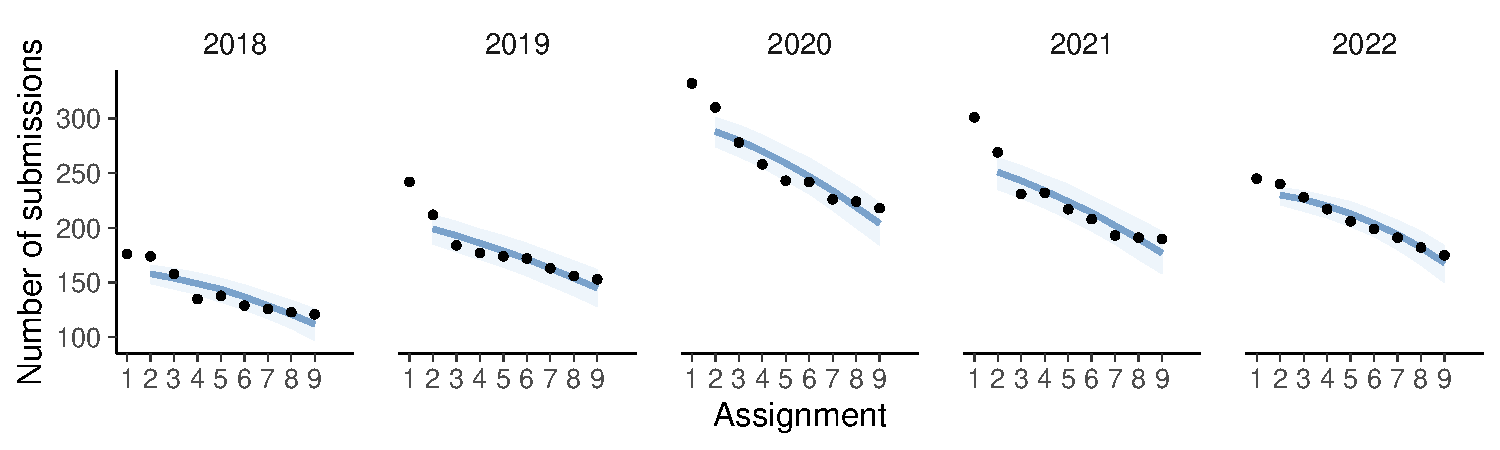
\includegraphics[height=3.6cm]{student_retention_lbinom_preds.pdf}
  \end{minipage}
  
\vspace{-0.25\baselineskip}  
Latent hierarchical linear model + spline\\  
  \hspace{-7mm}
  \begin{minipage}[t][3.6cm][t]{1.0\linewidth}
  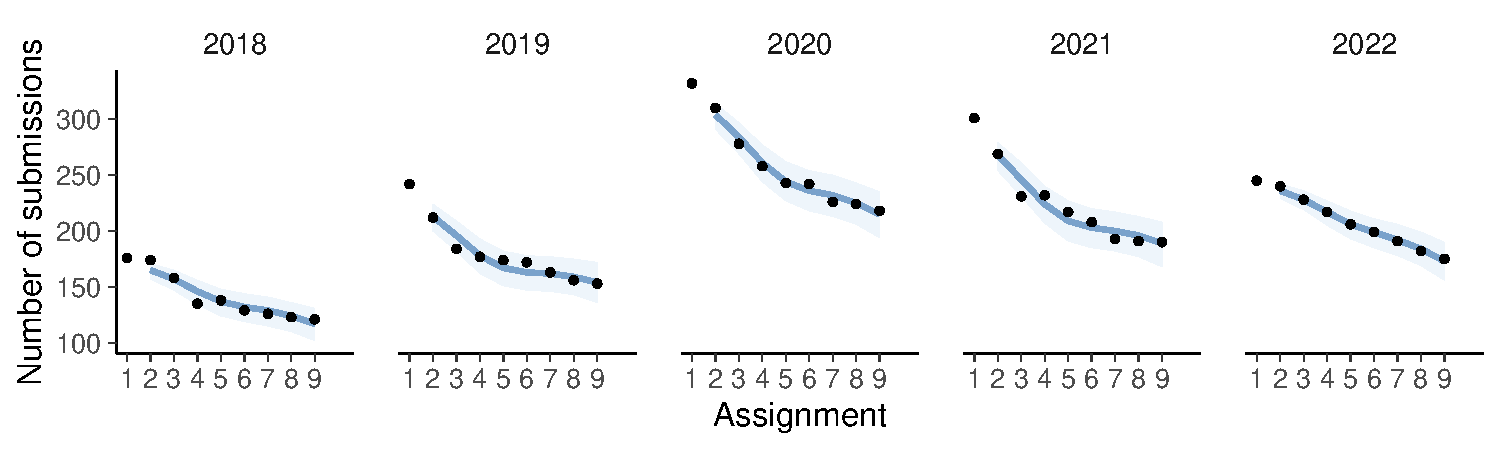
\includegraphics[height=3.6cm]{student_retention_sbinom_preds.pdf}
  \end{minipage}  

\end{frame}

\begin{frame}[fragile]{Student retention -- Marginal PPC}
\framesubtitle{\texttt{pp\_check(fit, ndraws=100)}}

  
\vspace{-0.75\baselineskip}  
Latent hierarchical linear model\\  
  \begin{minipage}[t][3.6cm][t]{1.0\linewidth}
    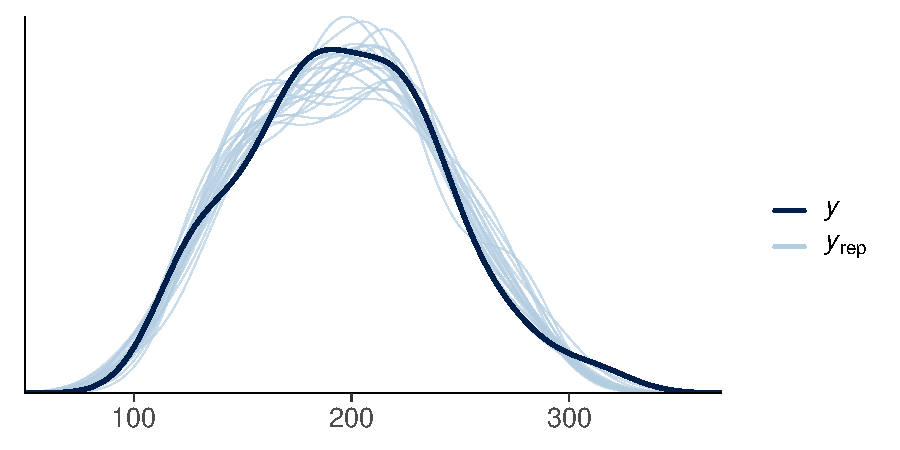
\includegraphics[height=3.6cm]{student_retention_lbinom_ppc_dens_overlay.pdf}
  \end{minipage}
  
\vspace{-0.5\baselineskip}  
Latent hierarchical linear model + spline\\  
  \begin{minipage}[t][3.6cm][t]{1.0\linewidth}
    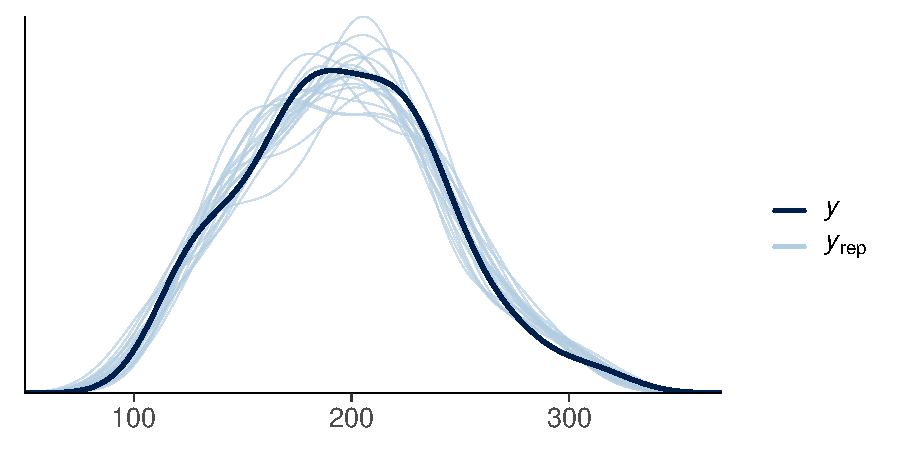
\includegraphics[height=3.6cm]{student_retention_sbinom_ppc_dens_overlay.pdf}
  \end{minipage}  

\end{frame}

\begin{frame}[fragile]{Student retention -- LOO intervals}

\vspace{-0.5\baselineskip}  
LOO predictive intervals -- latent hierarchical linear\\  
  \hspace{-7mm}
  \begin{minipage}[t][3.6cm][t]{1.0\linewidth}
    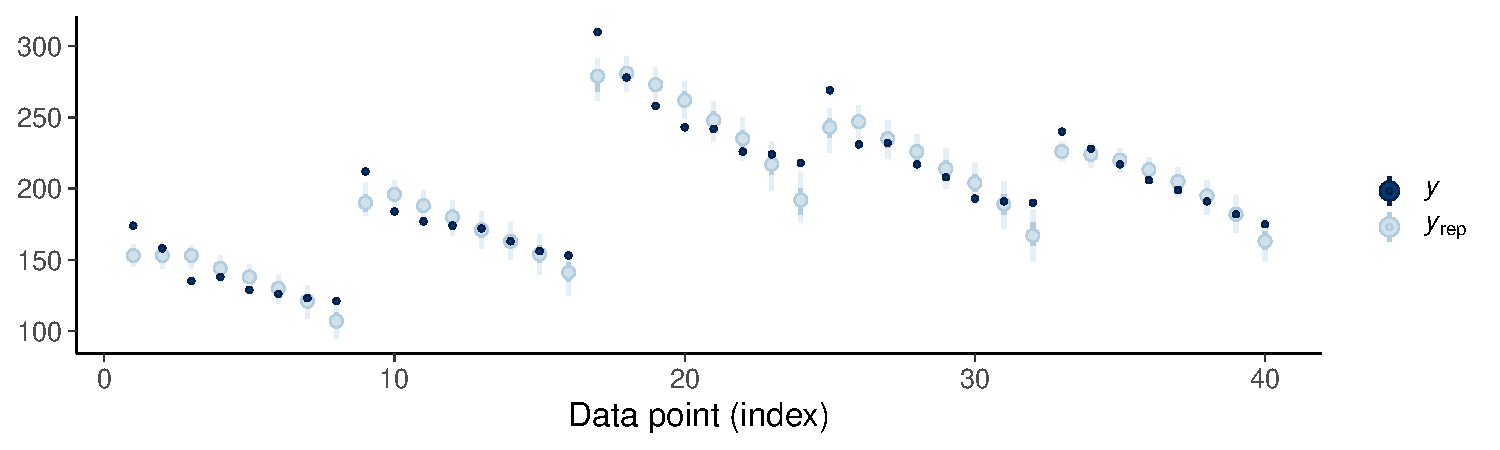
\includegraphics[height=3.6cm]{student_retention_lbinom_ppc_loo_intervals.pdf}
  \end{minipage}  

\vspace{-0.5\baselineskip}  
LOO predictive intervals -- latent hierarchical linear + spline\\  
  \hspace{-7mm}
  \begin{minipage}[t][3.6cm][t]{1.0\linewidth}
    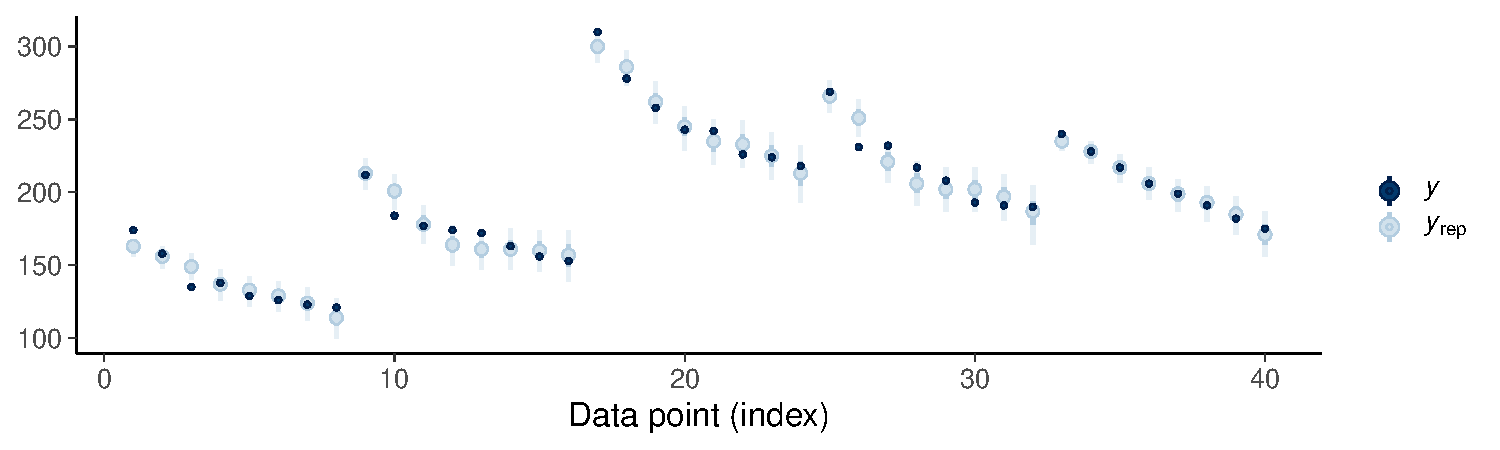
\includegraphics[height=3.6cm]{student_retention_sbinom_ppc_loo_intervals.pdf}
  \end{minipage}  

\end{frame}
  
\begin{frame}[fragile]{Student retention -- LOO-PIT checking}
\framesubtitle{\texttt{pp\_check(fit, type = "loo\_pit\_qq", ndraws=4000)}}

\vspace{-0.5\baselineskip}  
LOO-PIT check -- latent hierarchical linear\\  
  \hspace{-7mm}
  \begin{minipage}[t][3.6cm][t]{1.0\linewidth}
    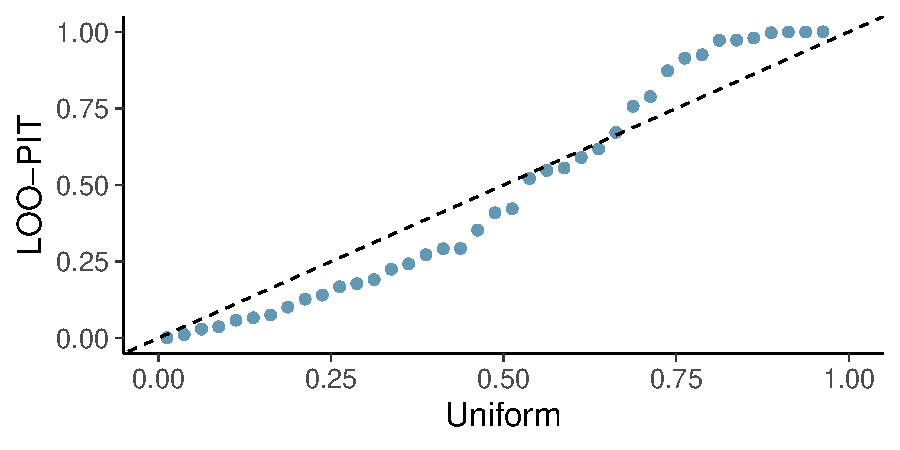
\includegraphics[height=3.6cm]{student_retention_lbinom_ppc_loo_pit_qq.pdf}
  \end{minipage}  

\vspace{-0.5\baselineskip}  
LOO-PIT check -- latent hierarchical linear + spline\\  
  \hspace{-7mm}
  \begin{minipage}[t][3.6cm][t]{1.0\linewidth}
    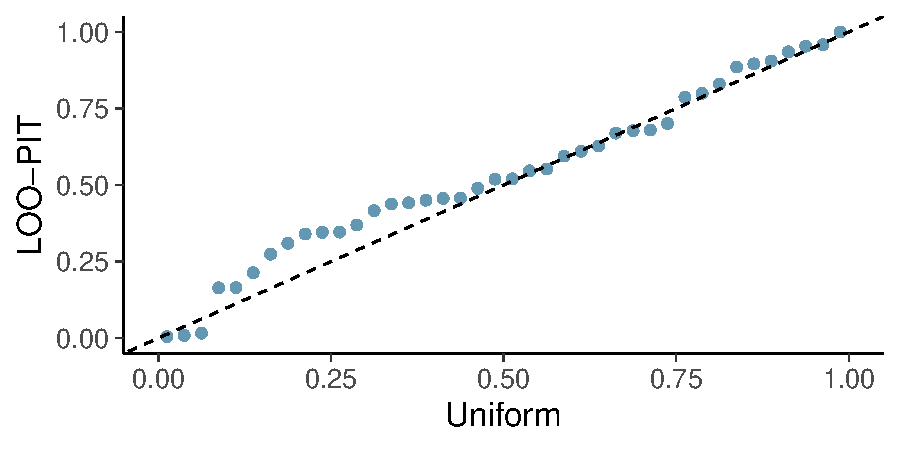
\includegraphics[height=3.6cm]{student_retention_sbinom_ppc_loo_pit_qq.pdf}
  \end{minipage}  

\end{frame}

\begin{frame}[fragile]{Student retention -- $R^2$}

Latent hierarchical linear vs. latent hierarchical linear + spline
  
\begin{minted}[fontsize=\footnotesize]{text}
> loo_R2(fit4) |> round(digits=2)
   Estimate Est.Error Q2.5 Q97.5
R2     0.92      0.02 0.88  0.95

> loo_R2(fit6) |> round(digits=2)
   Estimate Est.Error Q2.5 Q97.5
R2     0.97      0.01 0.95  0.98
\end{minted}

  $R^2$ measures the goodness of the mean of the predictive
  distribution

  \vspace{4\baselineskip}
{\color{gray}\footnotesize \href{https://doi.org/10.1080/00031305.2018.1549100}{Gelman, Goodrich, Gabry, and Vehtari (2019). R-squared for Bayesian regression models. \textit{The American Statistician}, 73(3):307-309.}}
  
\end{frame}

\begin{frame}[fragile]{Student retention -- log score -- elpd }

  \vspace{-\baselineskip}
  \begin{itemize}
  \item information theoretical goodness of the whole distribution
  \item elpd = expected log predictive density (probability)
  \item elpd\_loo = estimated with LOO predictive densities / probs\\
    $\sum_{n=1}^N \log p(y_i | x_i, x_{-i}, y_{-i})$
  \end{itemize}
 
% \vspace{-0.5\baselineskip}  
% LOO predictive intervals -- latent hierarchical linear\\  
%   \hspace{-7mm}
%   \begin{minipage}[t][3.6cm][t]{1.0\linewidth}
%     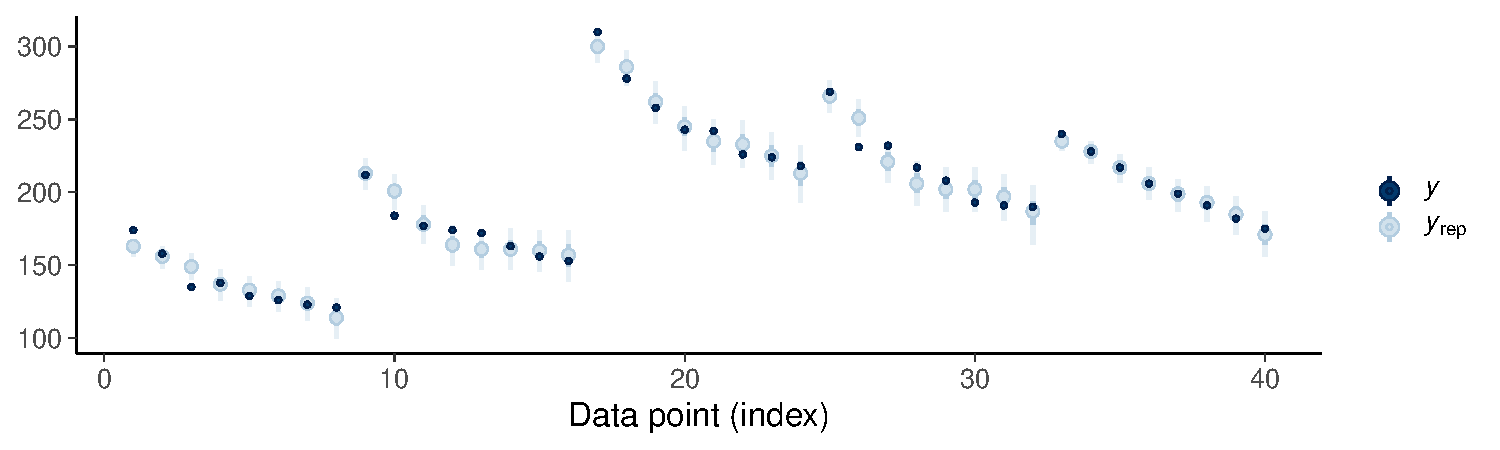
\includegraphics[height=3.6cm]{student_retention_sbinom_ppc_loo_intervals.pdf}
%   \end{minipage}  

%\vspace{-0.5\baselineskip}  
\only<2->{
  LOO predictive intervals -- latent hierarchical linear + spline\\  
  \begin{minipage}[t][3.6cm][t]{1.0\linewidth}
  \hspace{-9mm}
    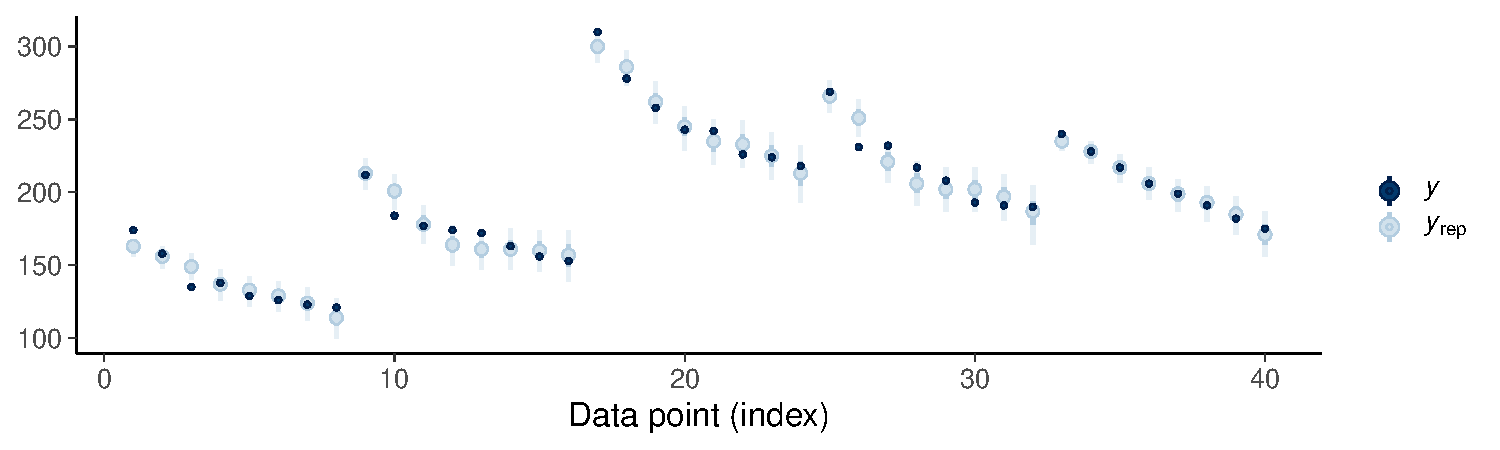
\includegraphics[height=3.6cm]{student_retention_sbinom_ppc_loo_intervals.pdf}
  \end{minipage}
}

\vspace{-1.75\baselineskip}
\only<3->{\fontsize{6.95}{9}\selectfont {~~~~~-8.4 -5.6 -2.9 -2.9 -2.8 -3.0 -4.0 -3.2 -3.9 -3.2 -3.4 -3.2 -2.9 -3.9 -3.4 -3.4 -3.2 -2.7 -2.8 -3.1\\
    ~~~~~~~~~-2.5 -2.8 -2.9 -3.4 -5.4 -3.7 -3.1 -3.3 -3.5 -3.2 -3.5 -3.5 -6.6 -3.8 -3.7 -3.4 -2.5 -2.8 -2.9 -3.3\\
  }}
\uncover<4->{\footnotesize $\sum = $ -141.7}
  
\end{frame}

\begin{frame}[fragile]{Student retention -- elpd\_loo}

Latent hierarchical linear + spline
\begin{minted}[fontsize=\footnotesize,highlightlines=6]{text}
> loo(fit6)

Computed from 4000 by 40 log-likelihood matrix

         Estimate   SE
elpd_loo   -141.7  7.2
p_loo        10.9  2.5
\end{minted}

\pause
Latent hierarchical linear
\begin{minted}[fontsize=\footnotesize,highlightlines=6]{text}
> loo(fit4)

Computed from 4000 by 40 log-likelihood matrix

         Estimate   SE
elpd_loo   -184.3 17.3
p_loo        24.3  5.8
\end{minted}

\end{frame}

\begin{frame}[fragile]{Student retention -- log score -- elpd }

  \vspace{-\baselineskip}
{
  {\small LOO predictive intervals -- latent hierarchical linear}\\  
  \begin{minipage}[t][2.8cm][t]{1.2\linewidth}
  \hspace{-9mm}
    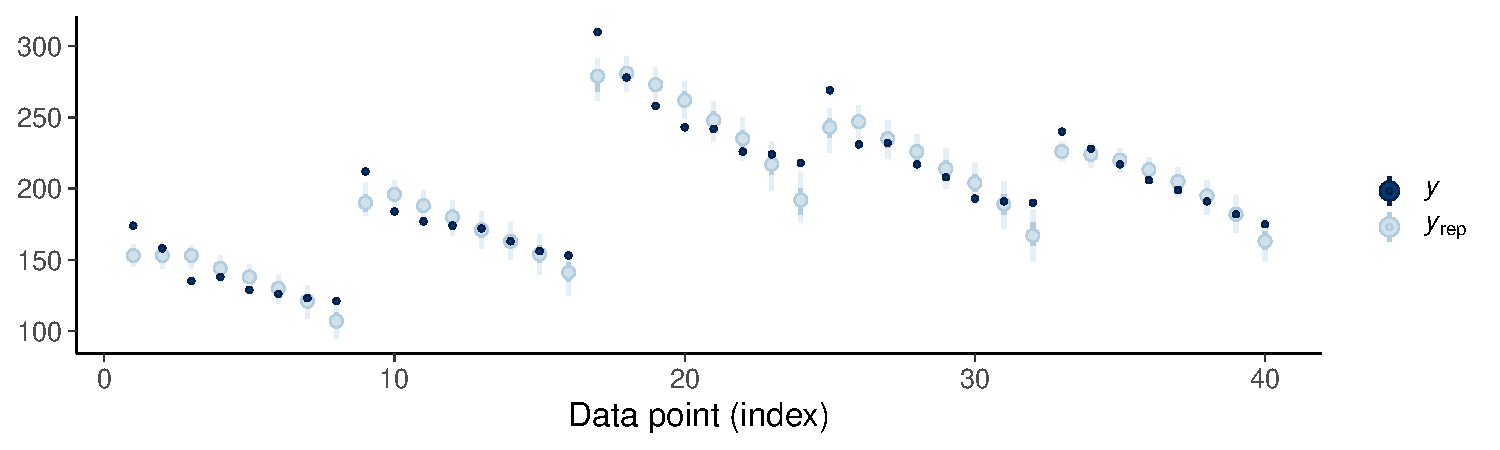
\includegraphics[height=2.8cm,trim=0 40 0 0,clip]{student_retention_lbinom_ppc_loo_intervals.pdf}
  \end{minipage}
}

\vspace{-1.75\baselineskip}
{\fontsize{6.7}{8}\selectfont {~~~~-15.7  -7.6  -3.9  -2.9  -6.7  -4.2  -2.9  -3.1 -12.9  -4.7  -3.3  -3.4 -9.0  -3.0  -3.3  -3.2  -8.2  -2.8  -3.2  -3.0\\
    ~~~~~~~~~-2.9 -3.3 -3.0 -4.6 -4.3 -3.3 -3.0 -4.0 -3.0 -5.6 -3.6 -5.4 -4.9 -3.6 -3.9 -5.2 -2.7 -3.7 -3.0 -4.1
  }}
{\scriptsize $\sum = $ -184.3}

{
  {\small LOO predictive intervals -- latent hierarchical linear + spline}\\
  \begin{minipage}[t][2.8cm][t]{1.2\linewidth}
  \hspace{-9mm}
    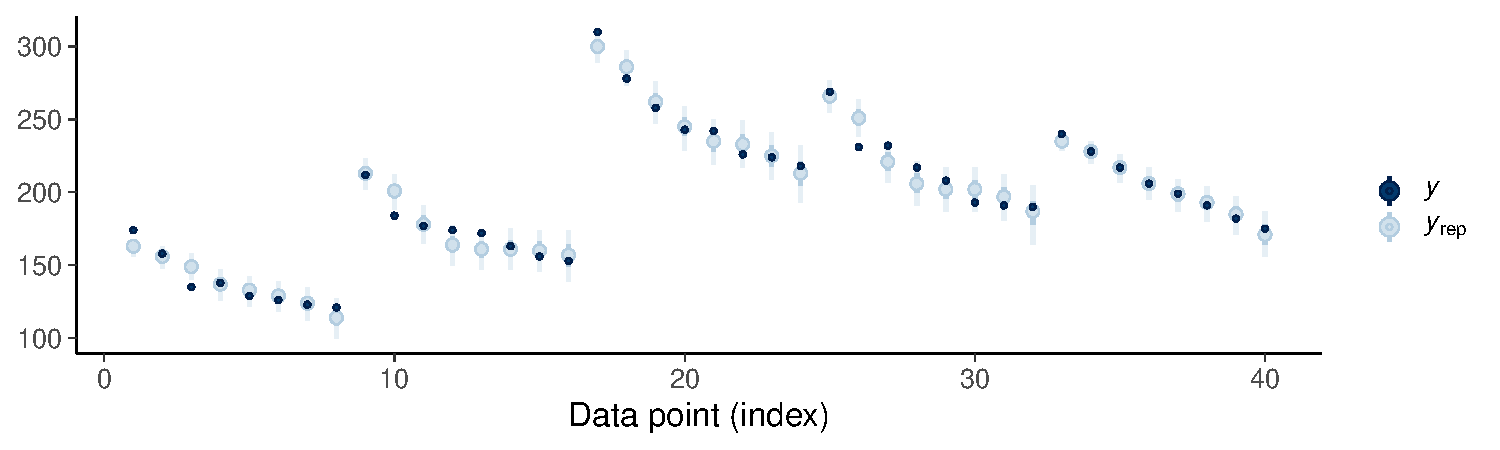
\includegraphics[height=2.8cm,trim=0 40 0 0,clip]{student_retention_sbinom_ppc_loo_intervals.pdf}
  \end{minipage}
}

\vspace{-1.75\baselineskip}
{\fontsize{6.7}{8}\selectfont {~~~~~-8.4 -5.6 -2.9 -2.9 -2.8 -3.0 -4.0 -3.2 -3.9 -3.2 -3.4 -3.2 -2.9 -3.9 -3.4 -3.4 -3.2 -2.7 -2.8 -3.1\\
    ~~~~~~~~~-2.5 -2.8 -2.9 -3.4 -5.4 -3.7 -3.1 -3.3 -3.5 -3.2 -3.5 -3.5 -6.6 -3.8 -3.7 -3.4 -2.5 -2.8 -2.9 -3.3
  }}
{\scriptsize $\sum = $ -141.7}
  
\end{frame}

\begin{frame}[fragile]{Student retention -- elpd\_loo}

  \vspace{-0.7\baselineskip}
  
\hspace{-5mm}Latent hierarchical linear (fit4) vs latent hierarchical linear + spline (fit6)

\only<+>{\hspace{-5mm}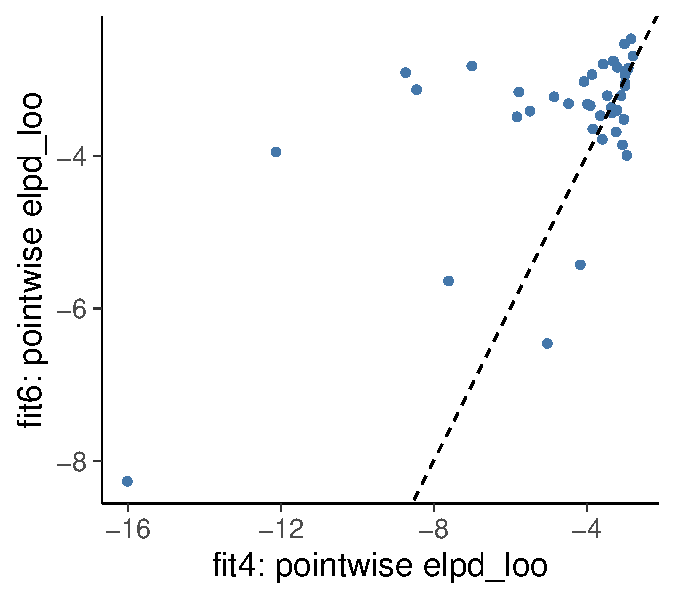
\includegraphics[height=7cm]{student_retention_loo_pointwise_scatter.pdf}}
\only<+>{\hspace{-5mm}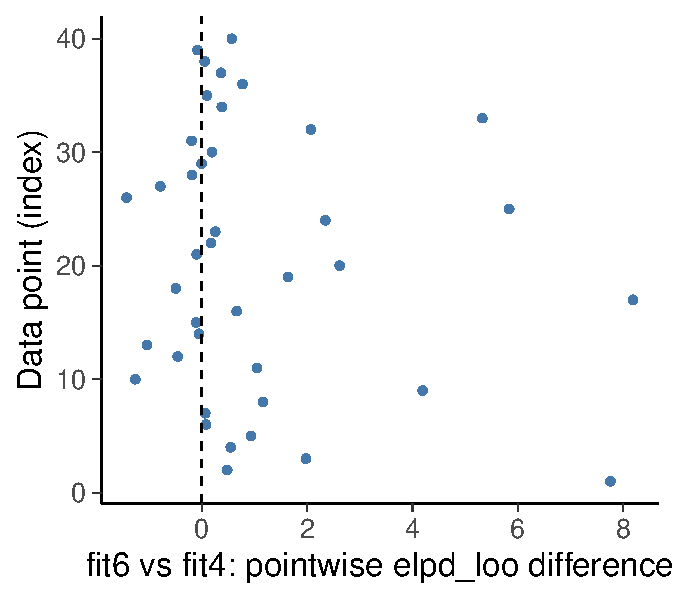
\includegraphics[height=7cm]{student_retention_loo_pointwise_diff_scatter.pdf}}
\only<+>{\hspace{-5mm}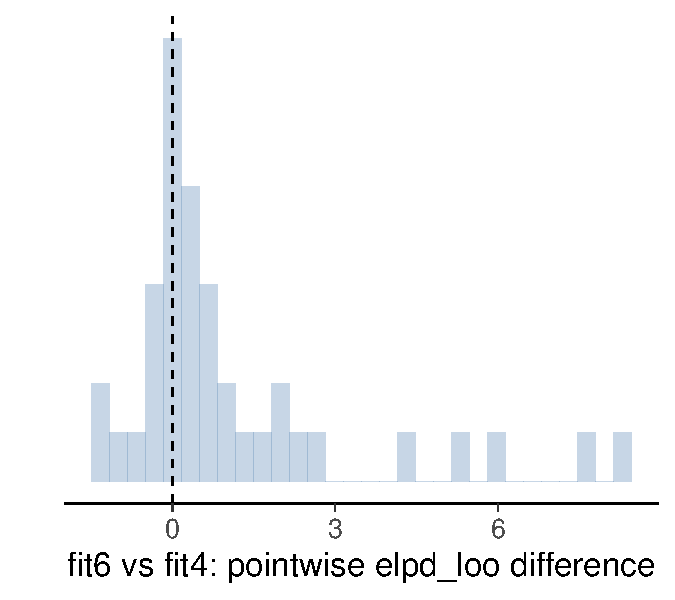
\includegraphics[height=7cm]{student_retention_loo_pointwise_diff_histogram_1.pdf}}
\only<+>{\hspace{-5mm}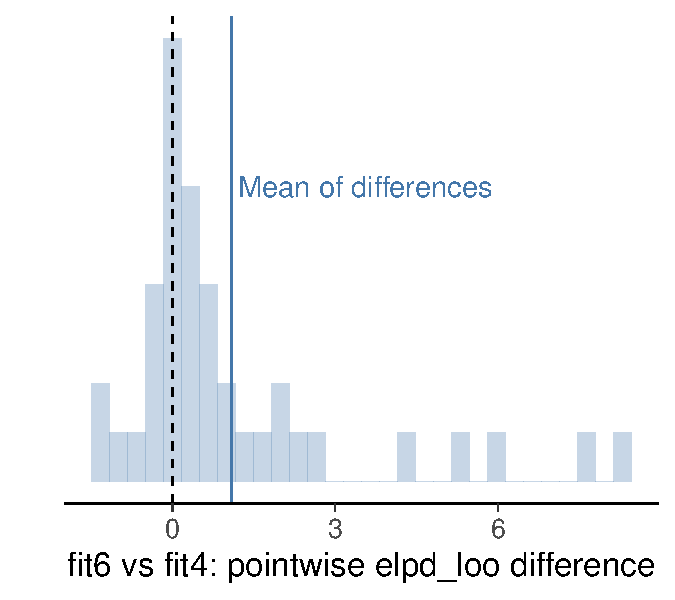
\includegraphics[height=7cm]{student_retention_loo_pointwise_diff_histogram_2.pdf}}
\only<+->{\hspace{-5mm}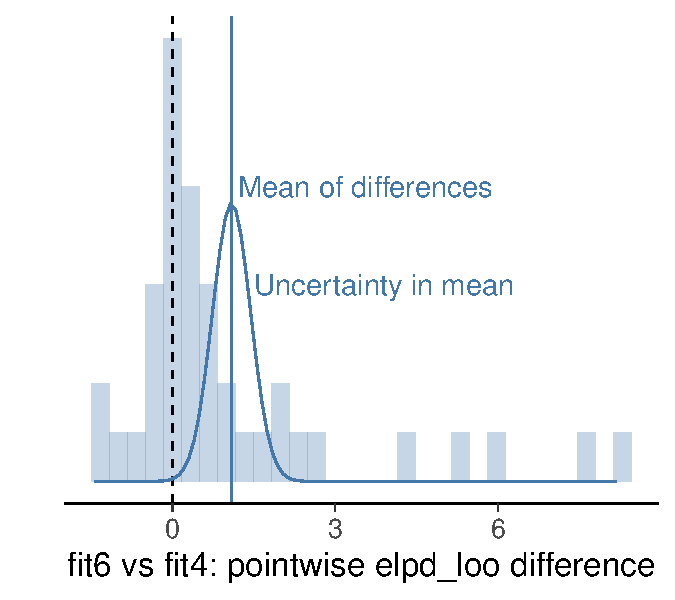
\includegraphics[height=7cm]{student_retention_loo_pointwise_diff_histogram_3.pdf}}
\only<+->{
  \begin{minipage}[t][4cm][t]{3.2cm}
    \vspace{-10.5\baselineskip}
    mean $\approx 1.07$\\
    \only<+->{sd $\approx 2.26$\\}
    \only<+->{SE = sd/$\sqrt{40}\approx 0.36$\\}
    \only<+->{\\sum $\approx 42.6$\\}
    \only<+->{SE = sd$*\sqrt{40}\approx 14.3$\\}
  \end{minipage}
}

\end{frame}

\begin{frame}[fragile]{Student retention -- elpd\_loo}

  {\color{gray}
Latent hierarchical linear + spline
\begin{minted}[fontsize=\footnotesize,highlightlines=3]{text}
> loo(fit6)
         Estimate   SE
elpd_loo   -141.7  7.2
p_loo        10.9  2.5
\end{minted}

Latent hierarchical linear
\begin{minted}[fontsize=\footnotesize,highlightlines=3]{text}
> loo(fit4)
         Estimate   SE
elpd_loo   -184.3 17.3
p_loo        23.8  5.7
\end{minted}
}

\begin{minted}[fontsize=\footnotesize,highlightlines={2-4}]{text}
> loo_compare(loo(fit4), loo(fit6))
     elpd_diff se_diff
fit6   0.0       0.0  
fit4 -42.6      14.3  
\end{minted}

\end{frame}

\begin{frame}{LOO difference uncertainty estimate (SE) reliability}
\vspace{-0.2\baselineskip}

  \begin{list1}
  \item[1.] The models make very similar predictions
    \begin{list2}
    \item<2-> if $|\mbox{elpd\_loo}|<4$, SE is not reliable, but the
      difference is small anyway
    \item<2-> selecting a ``wrong'' model has small cost
    \item<2-> in nested case, the skewness favors the simpler model
    \end{list2}
  \item[2.] The models are misspecified with outliers in the data
    \begin{list2}
    \item<3-> in nested case, the bias favors the simpler model
    \item<3-> model checking and model extension to avoid misspecified
      models (Bayesian workflow)
    \end{list2}
  \item[3.] The number of observations is small
    \begin{list2}
    \item<4-> in nested case the skewness favors the simpler model
    \item<4-> any inference with small $n$ is difficult
    \item<4-> if $|\mbox{elpd\_loo}|>4$, model is well specified,
      and $n>100$ then the normal approximation is good
    \end{list2}
  \end{list1}

{\color{gray}\footnotesize  Sivula, Magnusson, Matamoros, and Vehtari (2022). Uncertainty in Bayesian leave-one-out cross-validation based model comparison. \textit{\href{https://arxiv.org/abs/2008.10296v3}{arXiv:2008.10296v3}}.}
  
\end{frame}

\begin{frame}{Log score and elpd\_loo}

  \begin{itemize}
  \item Log score is not easily interpretable
  \item but is information theoretically good utility for the goodness
    of the whole distribution
  \item and thus is useful in model comparison
  \end{itemize}

\end{frame}

\begin{frame}{Log score and elpd\_loo}

  \begin{itemize}
  \item Interpretation in discrete case
    \begin{itemize}
    \item log probability
    \end{itemize}
  \item<2-> For example
    \begin{itemize}
    \item $\frac{1}{N}\sum_{n=1}^N\exp(\mathrm{elpd}_{\mathrm{loo},n}) \approx 4\%$ probability that we predict the
      observed value
    \item<3-> compare to guessing uniformly from the data range [121,310] having
      $1/(310-121+1) \approx 0.5\%$ probability \only<4->{(log score -210)}
    \end{itemize}
  \item<5-> Interpretation in continuous case
    \begin{itemize}
    \item can be compared to a simple reference distribution
    \end{itemize}
  \end{itemize}

\end{frame}

\begin{frame}{Assumptions about the future observations}

  \vspace{-\baselineskip}
  \only<1>{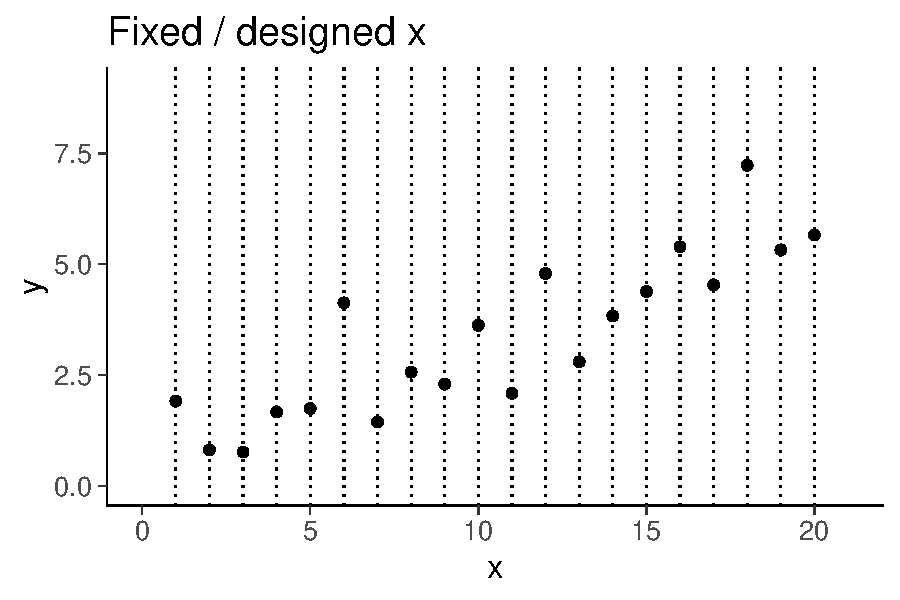
\includegraphics[width=9cm]{fakedfixed.pdf}}
  \only<2->{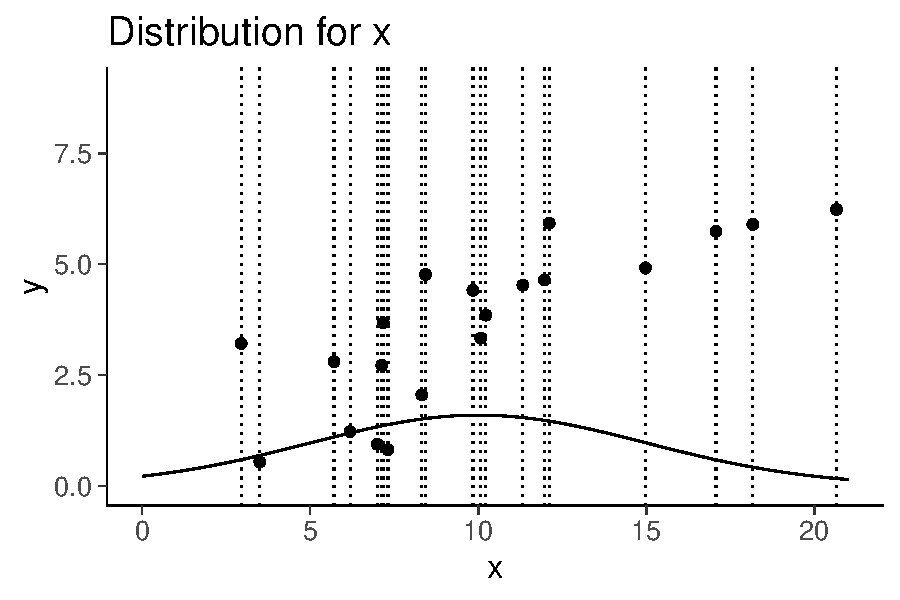
\includegraphics[width=9cm]{fakedrandom.pdf}}
  \\ 
  {\color{blue} $\mbox{elpd\_loo} = \sum_{i=1}^{20} \log p(y_i \mid x_i,x_{-i},y_{-i}) \approx -29.5$\\ \vspace{0.2\baselineskip}}
  {\color{blue} $\mbox{SE} = \sd(\log p(y_i \mid x_i,x_{-i},y_{-i}))\cdot \sqrt{20} \approx 3.3$\\}
  \vspace{0.5\baselineskip}
  \only<1>{LOO is ok for fixed / designed $x$. SE is uncertainty about $y \mid x$.\\\vspace{0.2\baselineskip}}\only<2->{LOO is ok for random $x$. SE is uncertainty about $y \mid x$ and $x$.\\\vspace{0.2\baselineskip}}\onslide<3>{Covariate shift handled with importance weighting or modelling}
  \onslide<1->{\\\vspace{\baselineskip} \small see \href{http://dx.doi.org/10.1214/12-SS102}{Vehtari \& Ojanen (2012)} and \href{https://users.aalto.fi/~ave/modelselection/CV-FAQ.html}{CV-FAQ}}
  
\end{frame}

\begin{frame}{Interpolation vs extrapolation}

  \only<1>{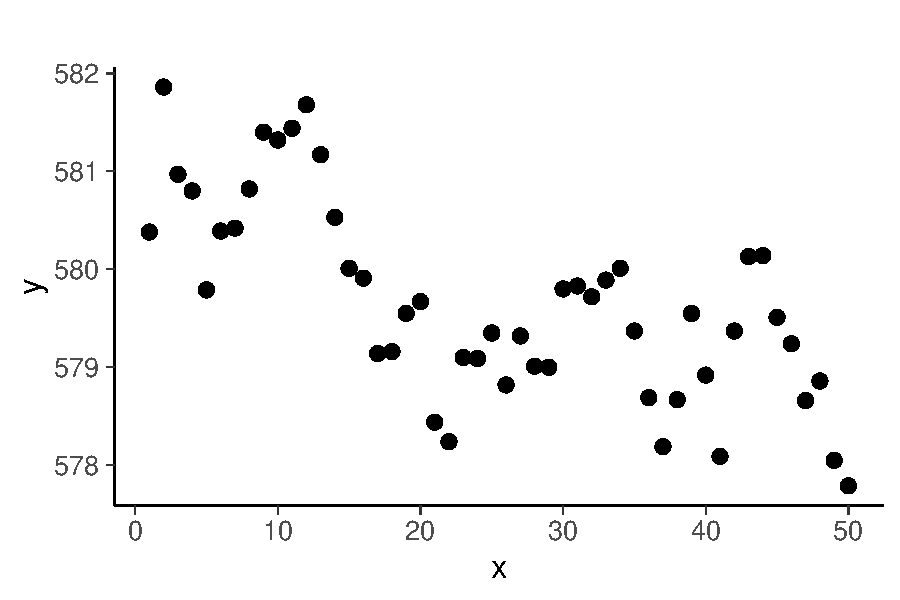
\includegraphics[width=9cm]{lake1data.pdf}}
  \only<2>{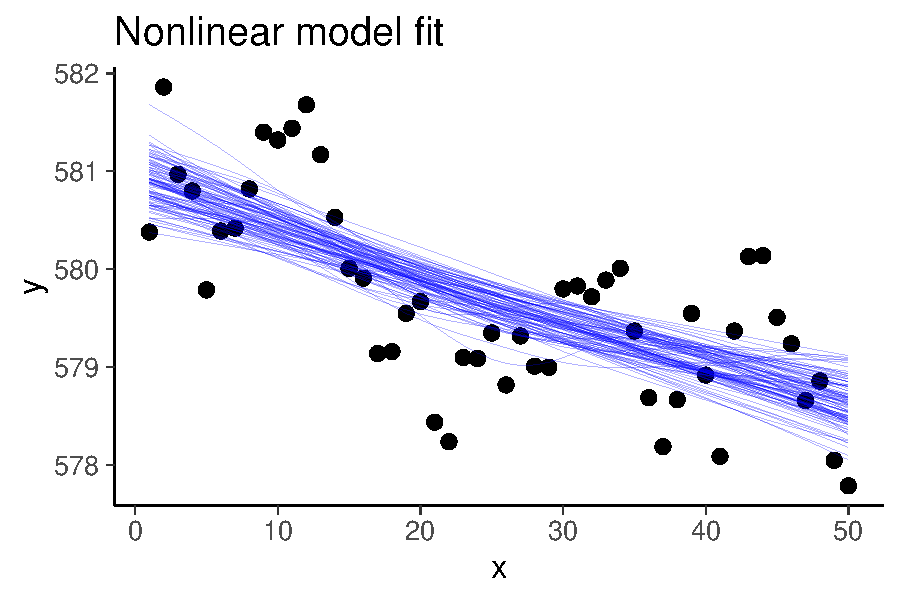
\includegraphics[width=9cm]{lake1gp.pdf}}
  \only<3->{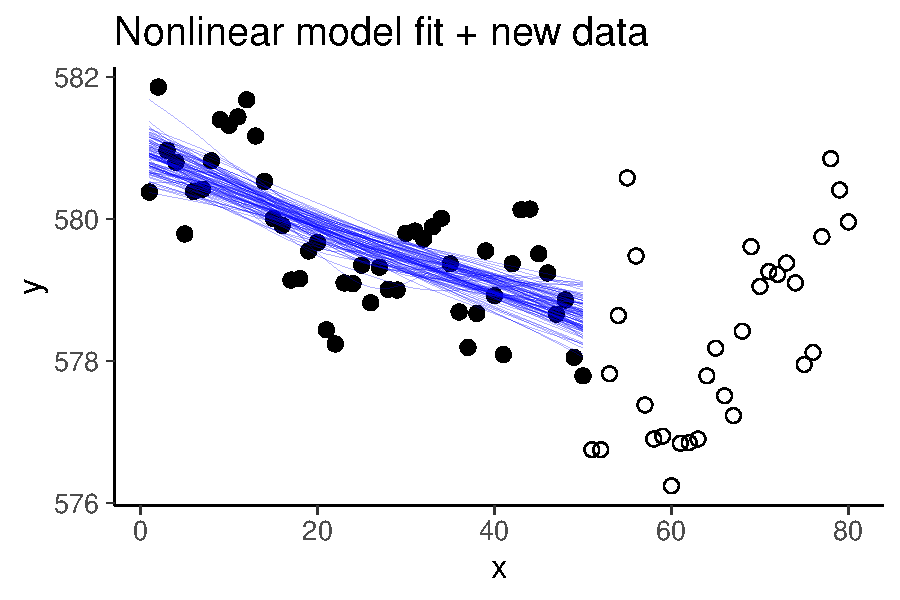
\includegraphics[width=9cm]{lake1gpptest.pdf}}
  \\
  \begin{itemize}
  \item<4> Extrapolation is more difficult
   item<5> In high dimensional case mostly extrapolation
  \end{itemize}
\end{frame}

\begin{frame}{Cross-validation for time series?}

  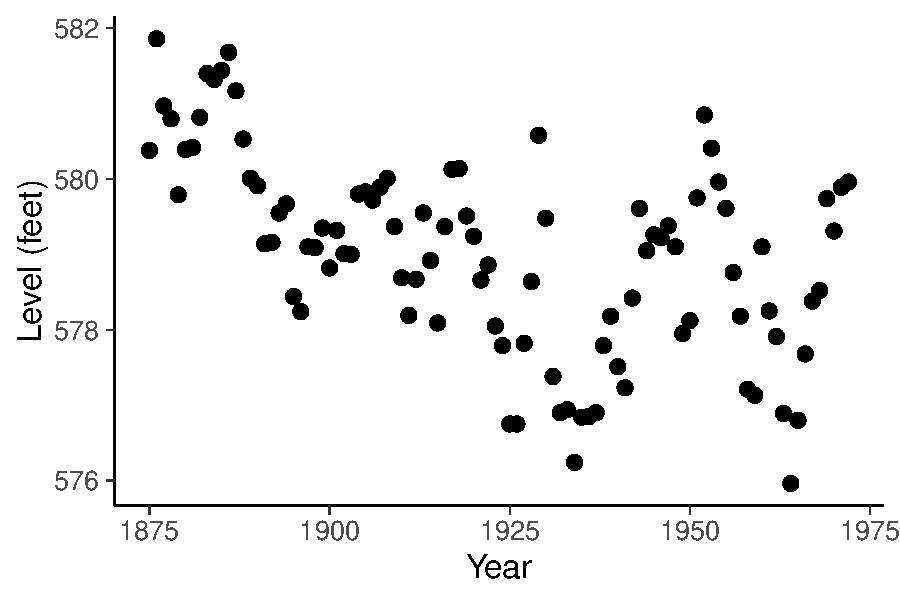
\includegraphics[width=9cm]{lake2data.pdf}

  
  {Can LOO or other cross-validation be used with time series?}
  
\end{frame}

\begin{frame}{Cross-validation for time series}

  \only<1>{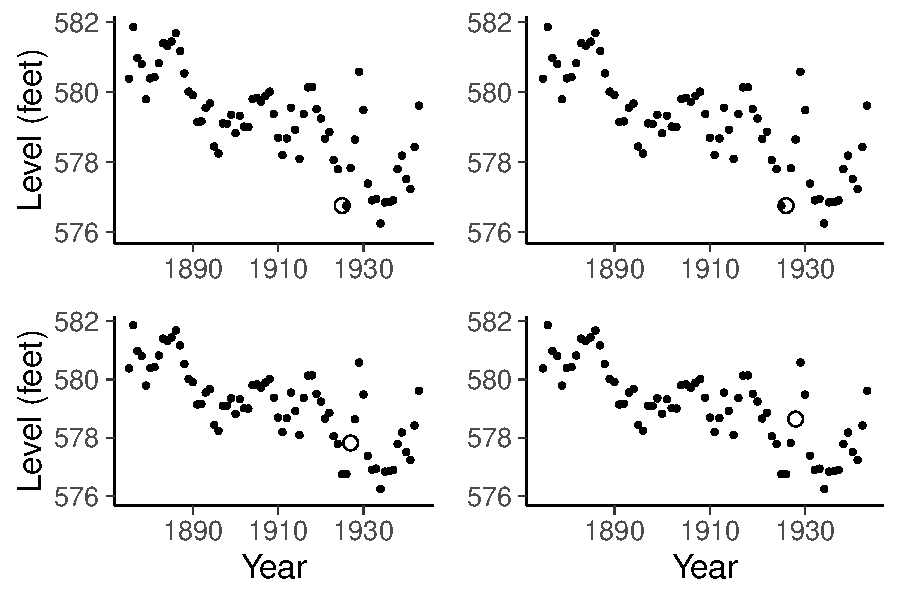
\includegraphics[width=9cm]{lake3loo.pdf}}
  \only<2>{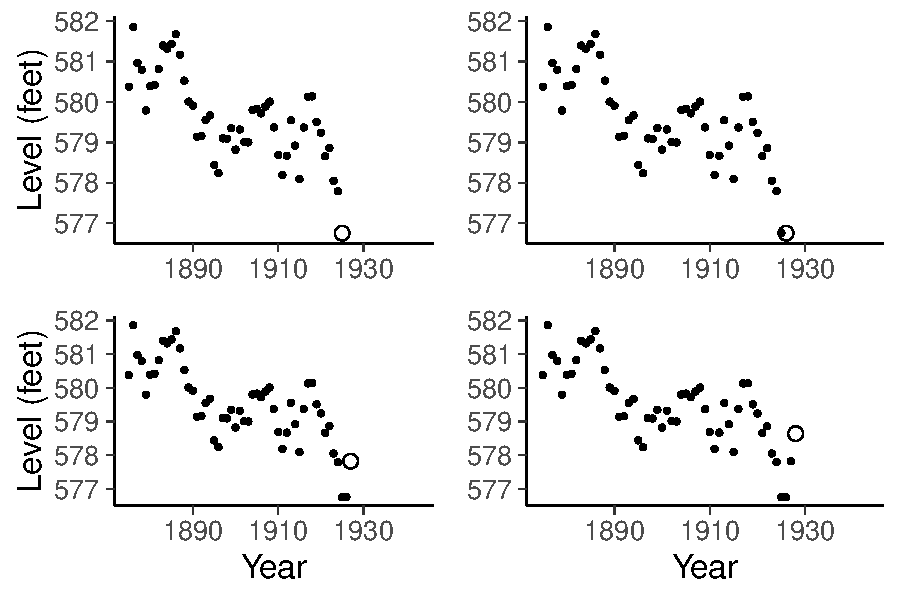
\includegraphics[width=9cm]{lake3stepahead.pdf}}
  \only<3>{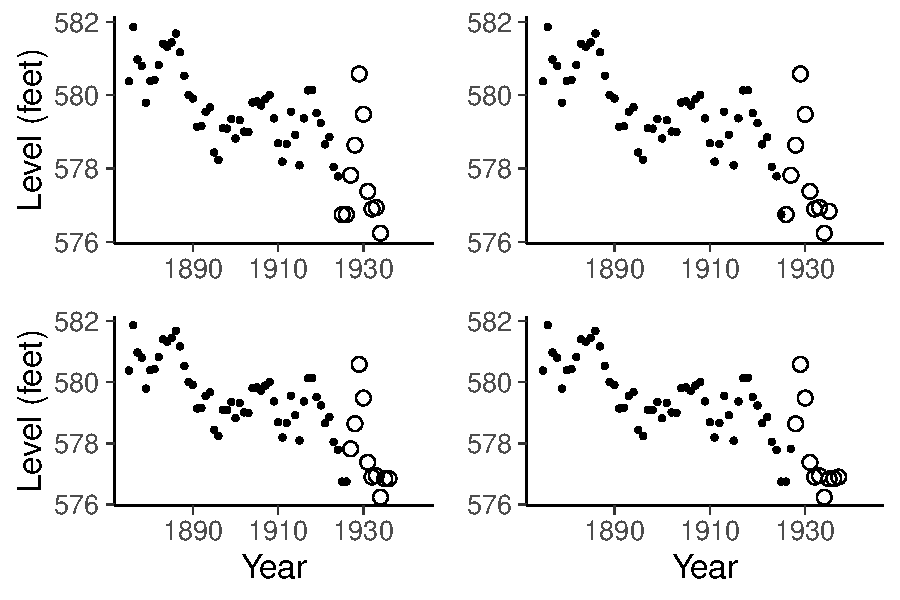
\includegraphics[width=9cm]{lake3tenstepahead.pdf}}
  \only<4>{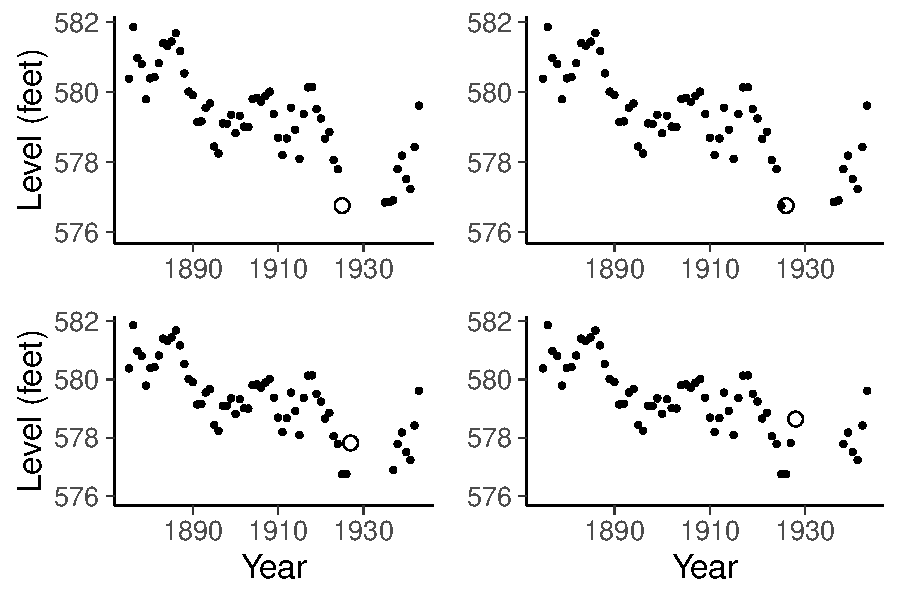
\includegraphics[width=9cm]{lake3stepaheadblock.pdf}}
  \\
  \only<1>{Leave-one-out cross-validation is ok for assessing conditional model}
  \only<2>{Leave-future-out (LFO) cross-validation is better for predicting future}
  \only<3>{$m$-step-ahead cross-validation is better for predicting further future}
  \only<4>{$m$-step-ahead leave-a-block-out cross-validation}
  
\end{frame}

\begin{frame}{Cross-validation for hierarchical data}

  \only<1>{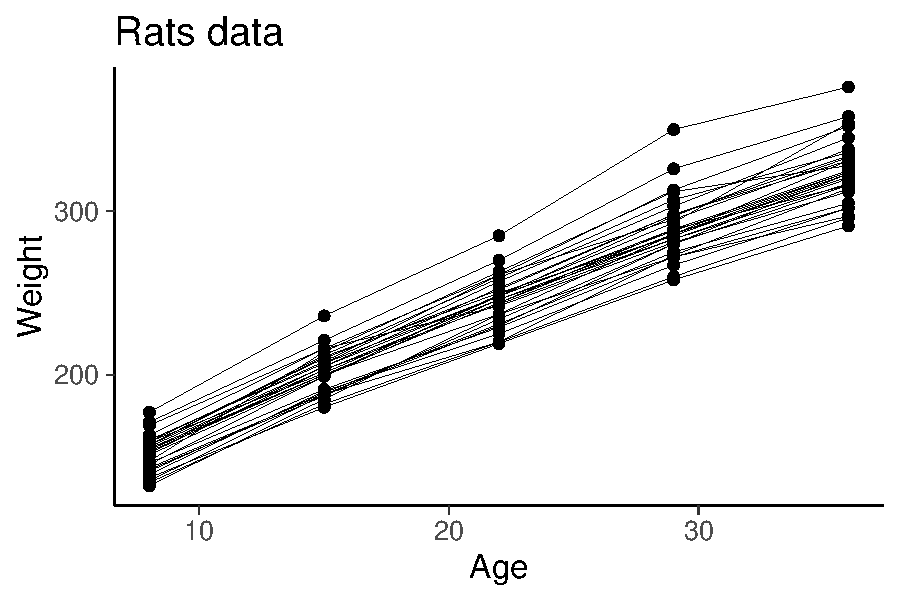
\includegraphics[width=9cm]{rats1data.pdf}}
  \only<2>{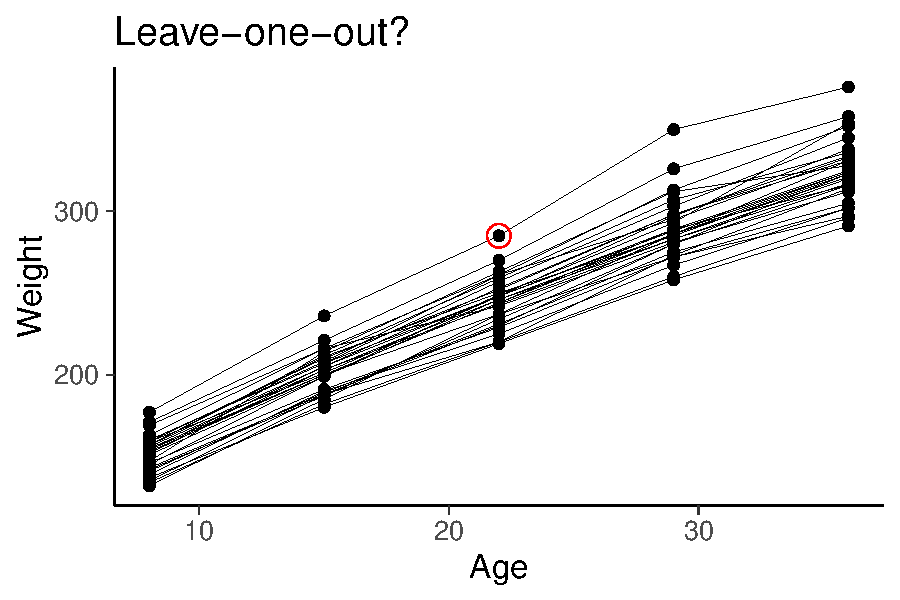
\includegraphics[width=9cm]{rats1loo.pdf}}
  \only<3>{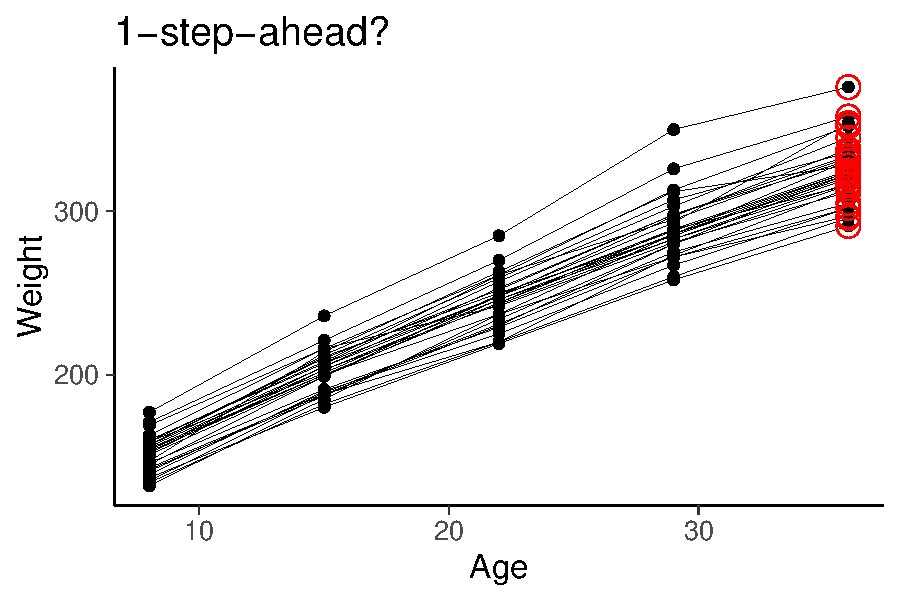
\includegraphics[width=9cm]{rats1step.pdf}}
  \only<4>{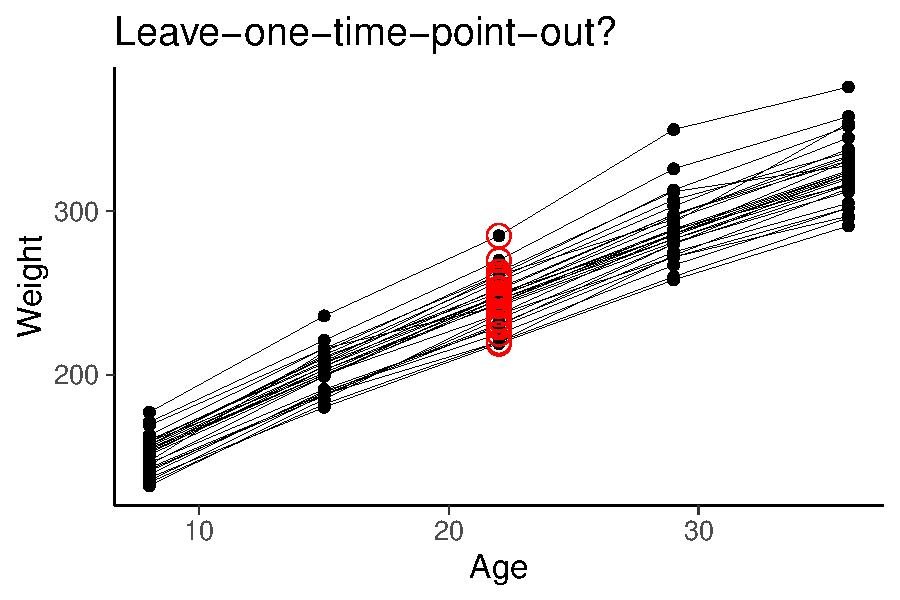
\includegraphics[width=9cm]{rats1onetime.pdf}}
  \only<5>{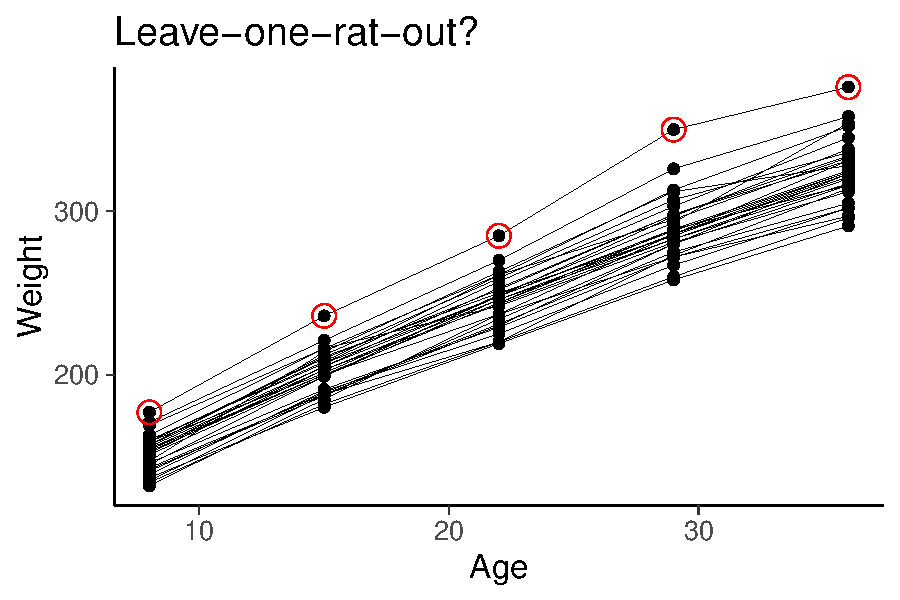
\includegraphics[width=9cm]{rats1onerat.pdf}}
  \only<6>{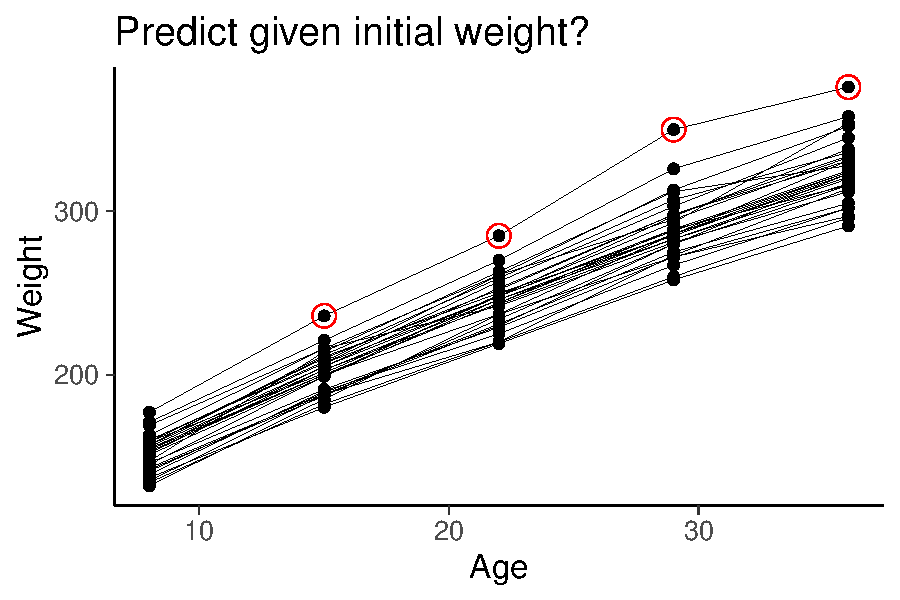
\includegraphics[width=9cm]{rats1init.pdf}}
  \\
  \only<1>{Can LOO or other cross-validation be used with hierarchical data?}
  \only<2->{Yes!}
  
\end{frame}

\begin{frame}{}

{\Large\color{navyblue} Summary of data generating mechanisms and prediction tasks}

\begin{list1}
\item You have to make some assumptions on data generating mechanism
\item Use the knowledge of the prediction task if available
\item Cross-validation can be used to analyse different parts, even if
  there is no clear prediction task
\end{list1}

\vspace{7.5\baselineskip}
{ \small see \href{http://dx.doi.org/10.1214/12-SS102}{Vehtari \& Ojanen (2012)} and \href{https://users.aalto.fi/~ave/modelselection/CV-FAQ.html}{CV-FAQ}}

\end{frame}

% \begin{frame}{LFO-CV}

%   \only<1>{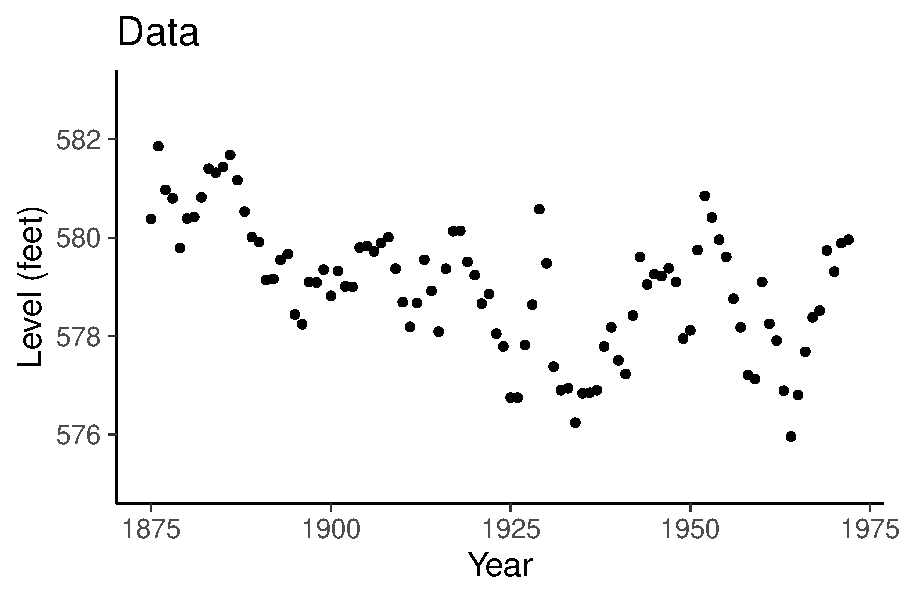
\includegraphics[width=9cm]{lake4data.pdf}}
%   \only<2>{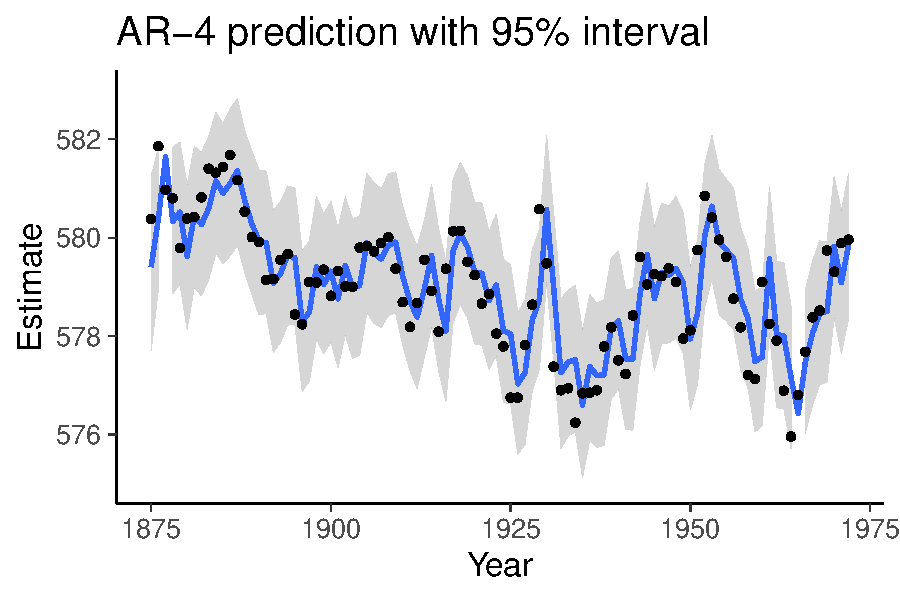
\includegraphics[width=9cm]{lake4pred.pdf}}
%   \only<3>{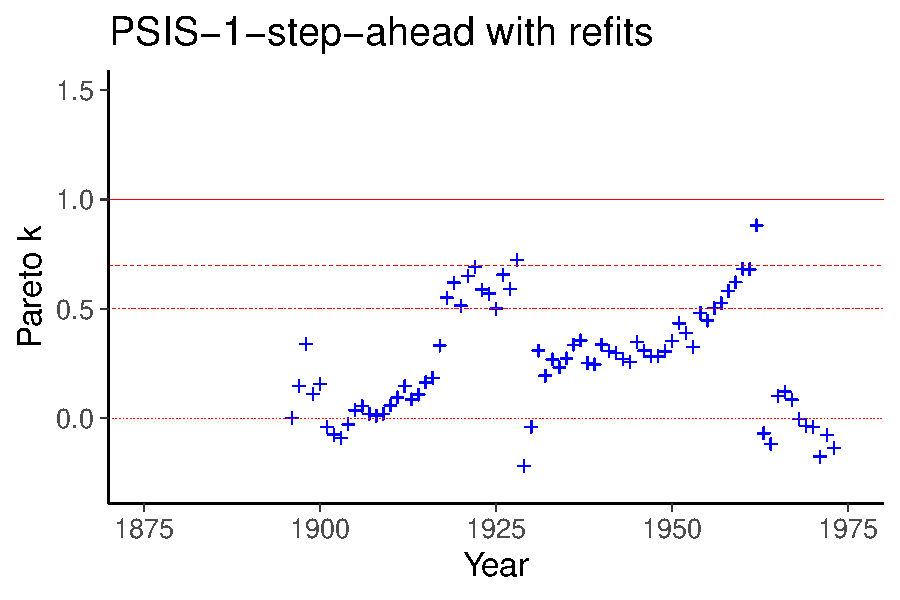
\includegraphics[width=9cm]{lake4psisrefits.pdf}}

%   \vspace{2\baselineskip}
%   \only<3> {\small \url{mc-stan.org/loo/articles/loo2-lfo.html}}

  
% \end{frame}

\begin{frame}{Pareto smoothed importance sampling CV variants}

\begin{list1}
\item PSIS-LOO for hierarchical models
  \begin{list2}
  \item leave-one-group out is challenging for PSIS-LOO\\ \vspace{0.2\baselineskip}
    
  \item Stan demo of the challenges and integrated LOO at \url{https://users.aalto.fi/~ave/modelselection/roaches.html}
  \item {\small see also Merkel, Furr and Rabe-Hesketh (2018)}
  \end{list2}
  \item<2-> PSIS-LOO for non-factorized models
    \begin{list2}
    \item {\url{mc-stan.org/loo/articles/loo2-non-factorizable.html}}
    \end{list2}
  \item<3-> PSIS-LOO for time series
  \begin{list2}
  \item Approximate leave-future-out cross-validation (LFO-CV) \\ \vspace{0.2\baselineskip}
    {\url{mc-stan.org/loo/articles/loo2-lfo.html}}
  \end{list2}
\end{list1}

\end{frame}


\begin{frame}{$K$-fold cross-validation}

\begin{list1}
\item $K$-fold cross-validation can approximate LOO
  \begin{list2}
    \item the same use cases as with LOO
  \end{list2}
\item $K$-fold cross-validation can be used for hierarchical models
  \begin{list2}
    \item good for leave-one-group-out
  \end{list2}
\item $K$-fold cross-validation can be used for time series
  \begin{list2}
    \item with leave-block-out
  \end{list2}
\end{list1}

\end{frame}

\begin{frame}{}

  \only<1>{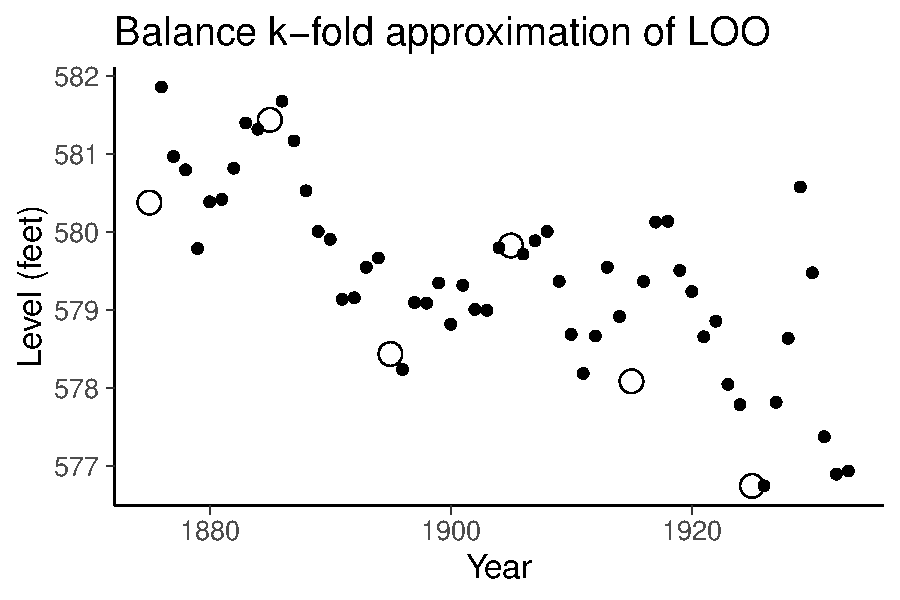
\includegraphics[width=10cm]{lake3kfoldbal1.pdf}} 
 \only<2>{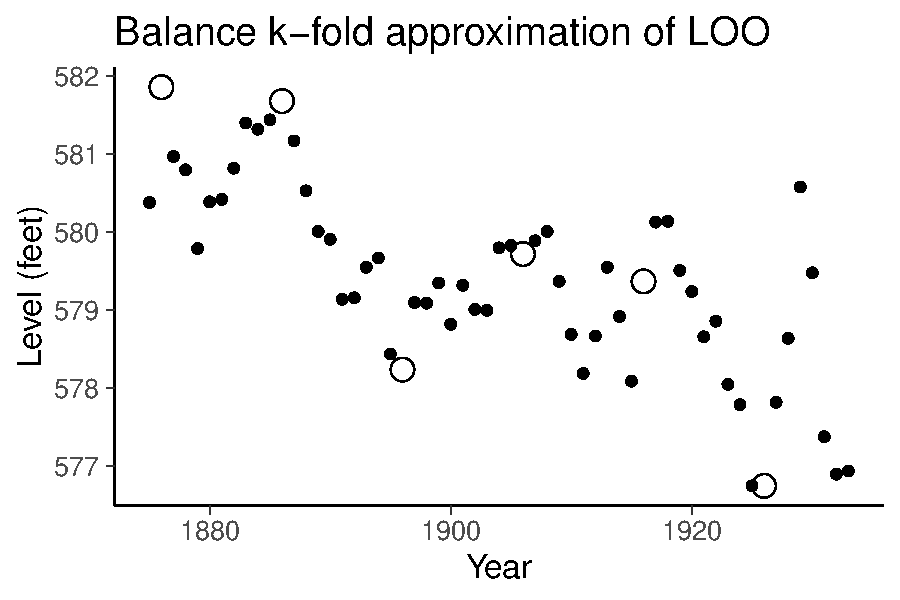
\includegraphics[width=10cm]{lake3kfoldbal2.pdf}}
  \only<3>{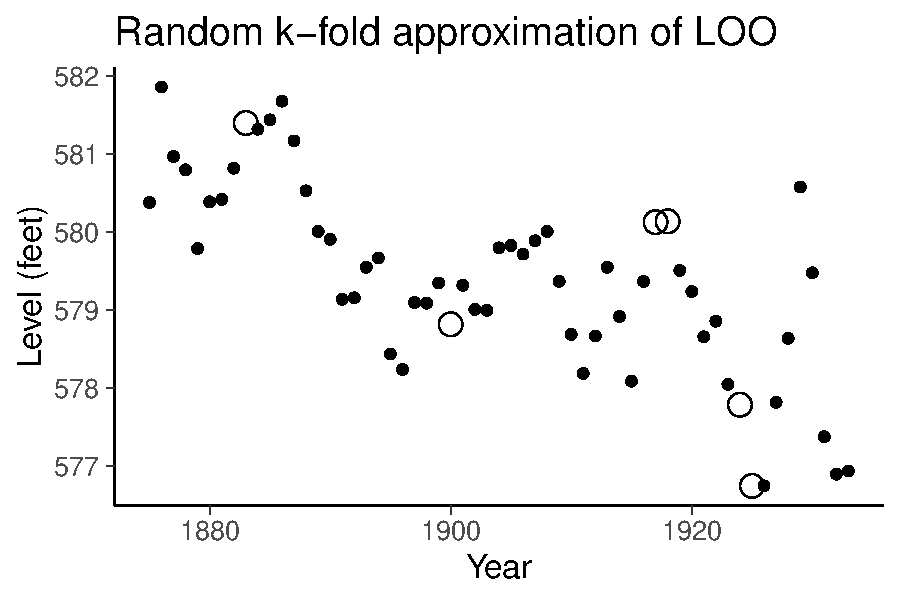
\includegraphics[width=10cm]{lake3kfoldrand.pdf}}
  \only<4>{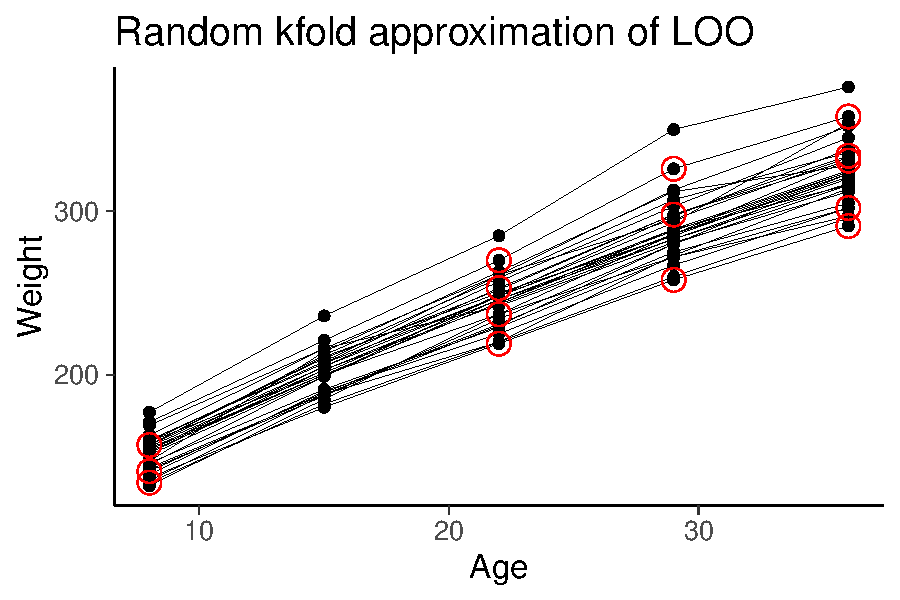
\includegraphics[width=10cm]{rats1kfoldrand.pdf}}
  \only<5->{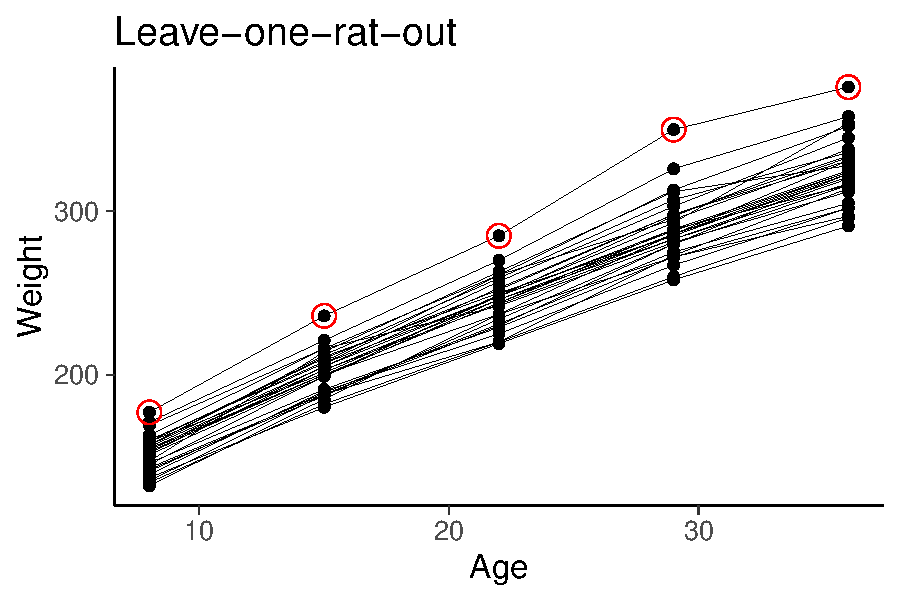
\includegraphics[width=10cm]{rats1oneratb.pdf}}
  % \\
  % \only<6>{kfold\_split\_random()\\ \vspace{0.2\baselineskip}
  % kfold\_split\_balanced()\\ \vspace{0.2\baselineskip}
  % kfold\_split\_stratified()}
  
\end{frame}

\begin{frame}{$K$-fold-CV code}

  \begin{list1}
  \item RStan, CmdStanR\\
    See vignette \url{http://mc-stan.org/loo/articles/loo2-elpd.html}
  \item RStanARM, brms\\
    \texttt{kfold(fit)}
  \item Alternative data divisions\\
  \rinline/kfold_split_random()/\\
  \rinline/kfold_split_balanced()/\\
  \rinline/kfold_split_stratified()/
  \end{list1}
  
\end{frame}


\begin{frame}[fragile]{looic?}

\begin{minted}[fontsize=\footnotesize,highlightlines={8}]{text}
> loo(fit6)

Computed from 4000 by 40 log-likelihood matrix

         Estimate   SE
elpd_loo   -141.7  7.2
p_loo        10.9  2.5
looic       283.4 14.4
------
Monte Carlo SE of elpd_loo is 0.1.
\end{minted}

  \begin{itemize}
  \item \rinline{loo} output shows also {looic}
  \item for historical non-Bayesian reasons it's -2 * elpd\_loo
    \begin{itemize}
      \item connection to deviance and information criteria
      \item you can just ignore it (I'd prefer it would not be shown)
    \end{itemize}

  \end{itemize}
  
\end{frame}

\begin{frame}{Information criteria}

  Information criteria estimate predictive performance, too
  
\begin{list1}
  \item<+-> AIC uses maximum likelihood estimate for prediction
  \item<+-> DIC uses posterior mean for prediction
  \item<+-> BIC is a simple approximation for marginal likelihood
  \item<+-> TIC, NIC, RIC, PIC, BPIC, QIC, AICc, ...
  \item<+-> WAIC is the only Bayesian information criterion
\end{list1}

\vspace{5\baselineskip}
{\color{gray}\footnotesize\href{http://dx.doi.org/10.1214/12-SS102}{Vehtari \& Ojanen (2012). A survey of Bayesian predictive methods for model assessment, selection and comparison. \textit{Statistics Surveys}, 6:142-228.}}
\end{frame}

\begin{frame}{WAIC vs PSIS-LOO}

\begin{list1}
  \item<+-> WAIC has the same target and assumptions as LOO
  \item<+-> PSIS-LOO is more accurate 
  \item<+-> PSIS-LOO has much better diagnostics
  \item<+-> moment matching and reloo are natural improvements for PSIS-LOO
  \item<5-> LOO makes the prediction assumption more clear,\\ which
    helps if $K$-fold-CV is needed instead
  \item<6-> Multiplying by -2 doesn't give any benefit\\ (Watanabe
    didn't multiply by -2)
\end{list1}

%\vspace{\baselineskip}
{\color{gray}\footnotesize \href{http://link.springer.com/article/10.1007/s11222-016-9696-4}{Vehtari, Gelman and Gabry (2017). Practical Bayesian model evaluation using leave-one-out cross-validation and WAIC. \textit{Statistics and Computing}, 27(5):1413–1432}\\
\href{http://dx.doi.org/10.1214/12-SS102}{Vehtari \& Ojanen (2012). A survey of Bayesian predictive methods for model assessment, selection and comparison. \textit{Statistics Surveys}, 6:142-228.}}

\end{frame}

\begin{frame}[fragile]{Marginal likelihood and Bayes factor}

  Bayes Factor $\frac{p(y|M_1)}{p(y|M_2)}$

  Marginal likelihood $p(y|M_1) = \int p(y|\theta,M_1)p(\theta|M_1)d\theta$

  \uncover<2->{
    Marginal likelihood with chain rule:\\
    $p(y|M_1) = p(y_1|M_1)p(y_2|y_1,M_1),\ldots,p(y_n|y_1,\ldots,y_{n-1},M_1)$\\
    \uncover<3->{where\\
      $p(y_1|M_1) = \int p(y_1|\theta,M_1)p(\theta|M_1)d\theta$\\
      $p(y_2|y_1,M_1) = \int p(y_2|\theta,M_1)p(\theta|y_1,M_1)d\theta$\\
      $\cdots$\\
      $p(y_n|y_1,\ldots,y_{n-1},M_1) = \int p(y_n|\theta,M_1)p(\theta|y_1,\ldots,y_{n-1},M_1)d\theta$\\
  } }

{\color{gray}\footnotesize
  \href{http://dx.doi.org/10.1214/12-SS102}{Vehtari \& Ojanen (2012). A survey of Bayesian predictive methods for model assessment, selection and comparison. \textit{Statistics Surveys}, 6:142-228.}\\
}

\end{frame}

\begin{frame}{Marginal likelihood / Bayes factor}

\vspace{-0.3\baselineskip}
\begin{list1}
\item Like leave-future-out 1-step-ahead cross-validation but starting with 0 observations\\
  \onslide<3->{- which makes it very sensitive to prior}
  \onslide<4->{and \\- unstable in case of misspecified
    models}\uncover<5->{ also asymptotically}
\end{list1}
\vspace{-0.5\baselineskip}
  \onslide<2->{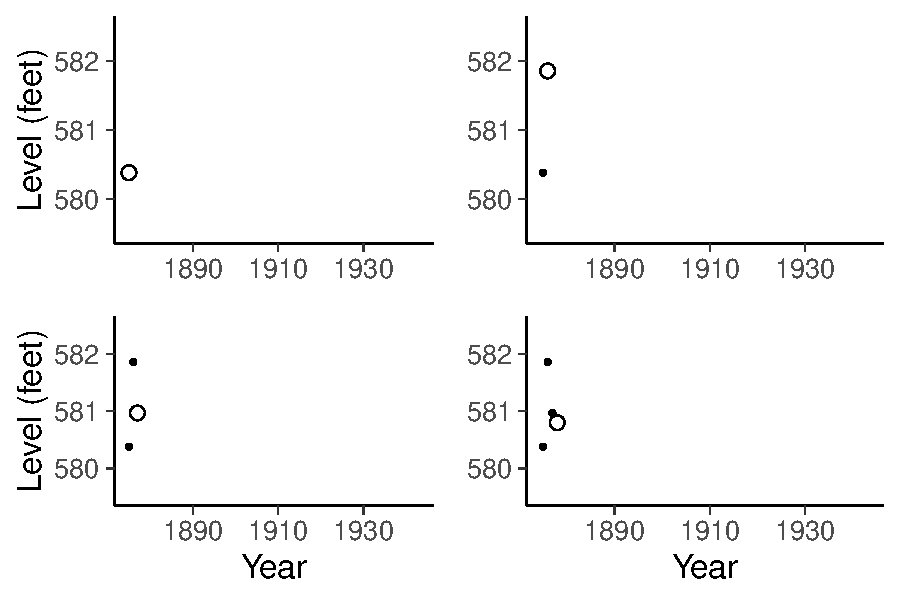
\includegraphics[width=9.4cm]{lake3bf.pdf}}

\end{frame}

\begin{frame}{Marginal likelihood / Bayes factor}

\vspace{-0.3\baselineskip}
\begin{list1}
\item Like leave-future-out 1-step-ahead cross-validation but starting with 0 observations\\
  {- which makes it very sensitive to prior}
  {and \\- unstable in case of misspecified
    models}{ also asymptotically}
\item Oelrich, Ding, Magnusson, Vehtari, and Villani (2020). When are Bayesian model probabilities overconfident? \textit{\href{https://arxiv.org/abs/2003.04026}{arXiv:2003.04026}}.
  
\end{list1}

\end{frame}

\begin{frame}{Predictive model selection}

  \begin{list1}
  \item Predictive model selection is most natural when the models are
    used for making predictions
  \item Predictive model selection can be also useful when the models
    are not directly used for prediction but for obtaining insights
    \begin{itemize}
    \item if there is no single independent parameter to look at
    \end{itemize}
  \item<2-> Student retention
    \begin{list2}
      \item latent hierarchical linear vs.
      \item latent hierarchical linear + spline
      \end{list2}
      is a good example where predictive model selection is useful
  \end{list1}

\end{frame}

\begin{frame}{Sometimes cross-validation is not needed}

\begin{list1}
\item<+-> In a simple nested case, often easier and more accurate to
  analyze posterior distribution of an independent parameter directly
  \begin{list2}
  \item instead of comparing\\
    \vspace{0.2\baselineskip}
    Model 1: $y \sim \normal(\alpha, \sigma)$\\
    \vspace{0.2\baselineskip}
    vs\\
    \vspace{0.2\baselineskip}
    Model 2: $y \sim \normal(\alpha + \beta x, \sigma)$\\
    \vspace{0.2\baselineskip}
    look at the posterior of $\beta$ directly
  \end{list2}
\item<+-> Randomized control treatment studies is natural example 
\end{list1}

\end{frame}

\begin{frame}{Common statistical tests as Bayesian models}

  \begin{itemize}
  \item Most common statistical tests are linear models\\
    \vspace{0.5\baselineskip}
    \hspace{-0.8cm}\begin{minipage}[t]{1.0\linewidth}
      {\small
        \begin{tabular}{lll}
          test & model & formula \\\hline
          $t$-test & mean of data & \rinline/y ~ 1/\\
          paired $t$-test & mean of diffs &\rinline/(y1 - y2) ~  1/\\
          Pearson correl. & linear model &\rinline/y ~  1 + x/\\
          two-sample $t$-test & group means &\rinline/y ~  1 + gid/\\
          ANOVA & hier. model &\rinline/y ~  1 + (1 | gid)/\\
          $\ldots$ &
        \end{tabular}}
      \end{minipage}
  \item<2->  Possible to extend, e.g., with group specific variances and and
    different distributions such $t$- or Poisson distribution
    \begin{itemize}
    \item and go beyond named tests
    \end{itemize}
  \item<3-> See longer list and illustrations (with {\tt lm}) at
  \url{https://lindeloev.github.io/tests-as-linear/}\\
  and\\
  with rstanarm in \href{https://avehtari.github.io/ROS-Examples/}{Regression and other stories}
\end{itemize}

\end{frame}

\begin{frame}[fragile]{Beta blockers}

\begin{itemize}
  \item An experiment was performed to estimate the effect of
    beta-blockers on mortality of cardiac patients
  \item A group of
    patients were \textit{randomly} assigned to \textit{control} and \texttt{treatment} groups:
    \begin{itemize}
    \item out of 674 patients receiving the control, 39 died
    \item out of 680 receiving the treatment, 22 died
    \end{itemize}
  \end{itemize}

\end{frame}

\begin{frame}[fragile]{Beta blockers}

\begin{itemize}
  \item An experiment was performed to estimate the effect of
    beta-blockers on mortality of cardiac patients
  \item A group of
    patients were randomly assigned to treatment and control groups:
    \begin{itemize}
    \item out of 674 patients receiving the control, 39 died
    \item out of 680 receiving the treatment, 22 died
    \end{itemize}
  \end{itemize}

\begin{minted}[fontsize=\footnotesize,escapeinside=\%\%]{r}
d_bin2 <- data.frame(N = c(674, 680),
                     y = c(39,22),
                     grp2 = c(0,1))

fitb1 <- brm(%\highlight{y | trials(N) ~ 1}%, family = binomial(), data = d_bin2)

fitb2 <- brm(%\highlight{y | trials(N) ~ 1 + grp2}%, family = binomial(), data = d_bin2)
\end{minted}
  \pause
\begin{minted}[fontsize=\footnotesize,escapeinside=\%\%]{r}
> loo_compare(loo(fitb1),loo(fitb2))
      elpd_diff se_diff
fitb2  0.0       0.0   
fitb1 -1.6       2.3   
\end{minted}
\end{frame}

\begin{frame}{Posterior inference}

  \begin{itemize}
  \item Instead of model selection, report full posterior \only<1>{and}
    \begin{itemize}
      \only<1>{
      \item<1> compare to expert information
      \item<1> combine with utility/cost function
      }
      \only<2>{
      \item for continuous posterior there is zero probability that
        e.g. treatment effect is exactly zero
      }
      \only<3>{
      \item for continuous posterior we could report the probability
        that we know the sign of the effect
      }
    \end{itemize}
  \end{itemize}
  
  \only<1>{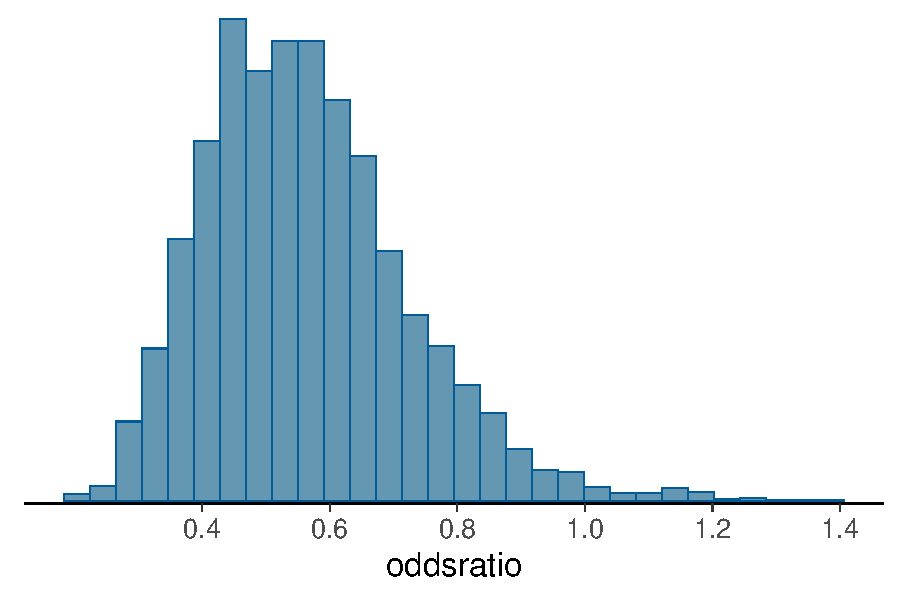
\includegraphics[width=10cm]{odds1_fullp.pdf}}
  \only<2>{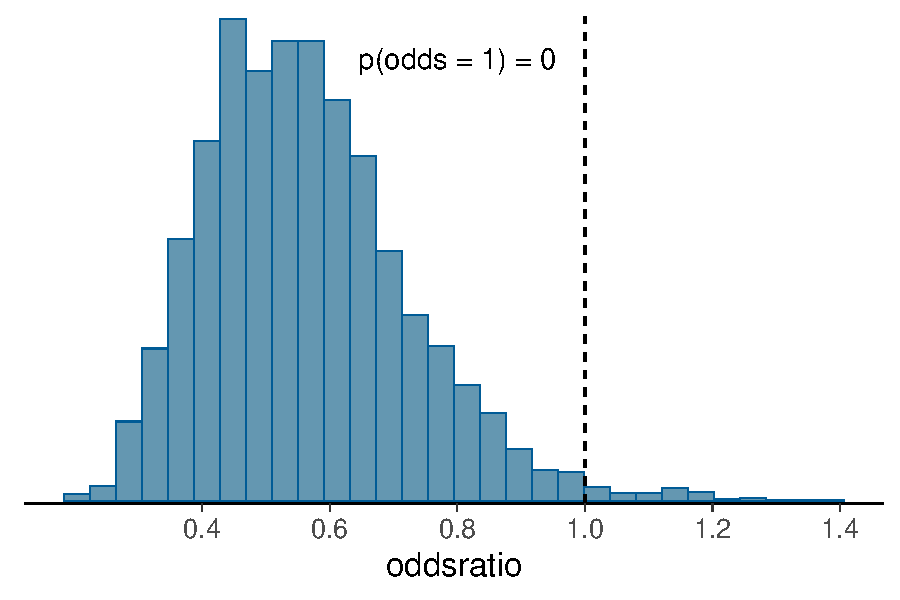
\includegraphics[width=10cm]{odds1_eq.pdf}}
  \only<3>{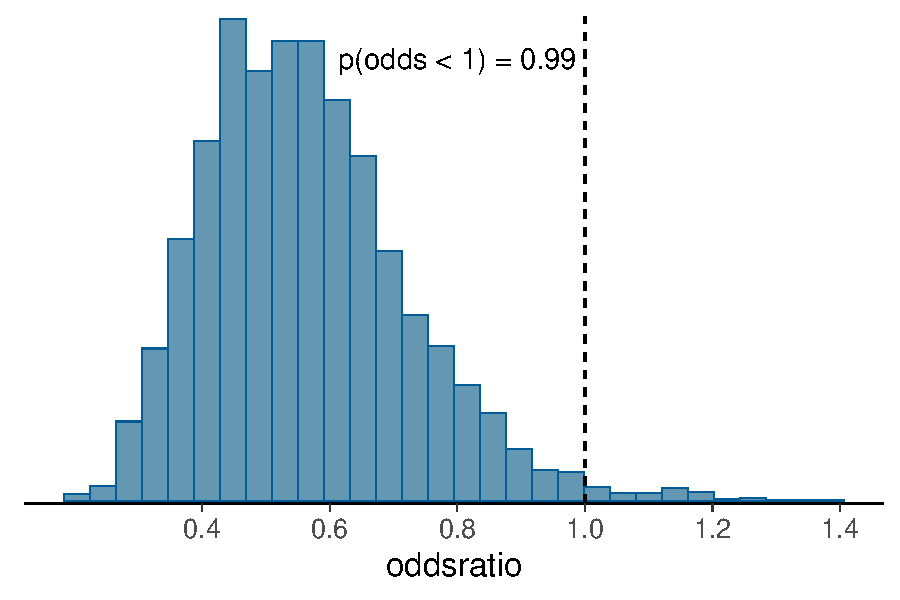
\includegraphics[width=10cm]{odds1_less.pdf}}
  
\end{frame}

\begin{frame}{Bayesian hypothesis testing}

  \begin{itemize}
  \item Sometimes people want to make a dichotomous choice
    \begin{itemize}
    \item model selection
    \item hypothesis testing
    \end{itemize}
  \item<2-> For example, need to make a decision whether continue with
    bigger clinical trials or give permission to sell a drug
    \begin{itemize}
    \item the first decision requires estimates of trial costs and
      sales profits, too
    \item the second decision is based on safety
    \item more abiut decision analysis next week
    \end{itemize}
  \item<3-> Now we look at idealized hypothesis testing
  \end{itemize}

\end{frame}

\begin{frame}{Bayesian hypothesis testing}

  \begin{itemize}
  \item Instead of model selection, report full posterior {and}
    \begin{itemize}
      \item for continuous posterior some people compare whether
        posterior interval includes null case
    \end{itemize}
  \end{itemize}
  
  {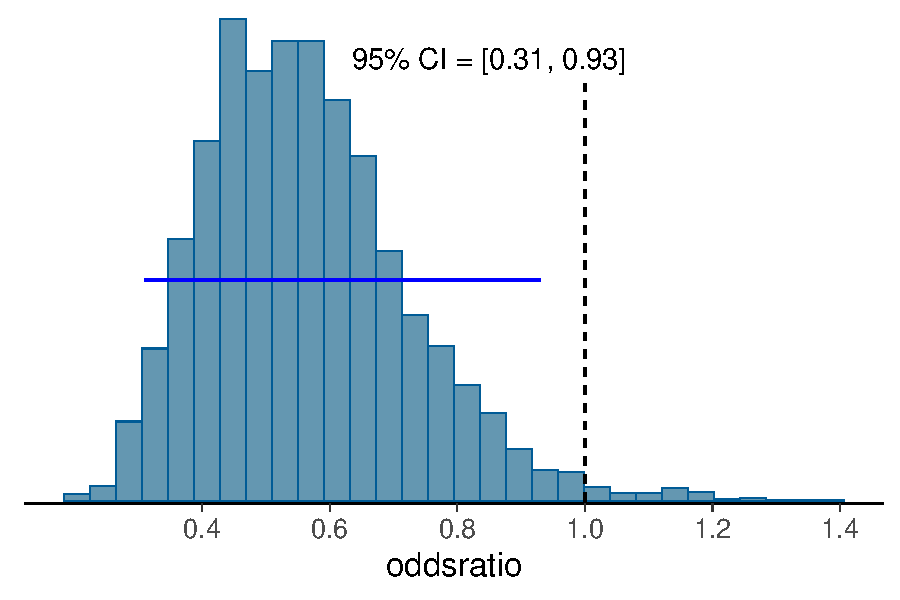
\includegraphics[width=10cm]{odds1_ci.pdf}}
  
\end{frame}

\begin{frame}{Bayesian hypothesis testing}

  \begin{itemize}
  \item Equivalence testing (region of practical equivalence)
    \begin{itemize}
    \item what is the probability that the effect is closer than
      $\epsilon$ to null, where $\epsilon$ is based on what is
      practically useful effect size
      % \only<2>{
      % \item some people combine posterior interval and region of
      %   practical equivalence}
    \end{itemize}
  \end{itemize}

    {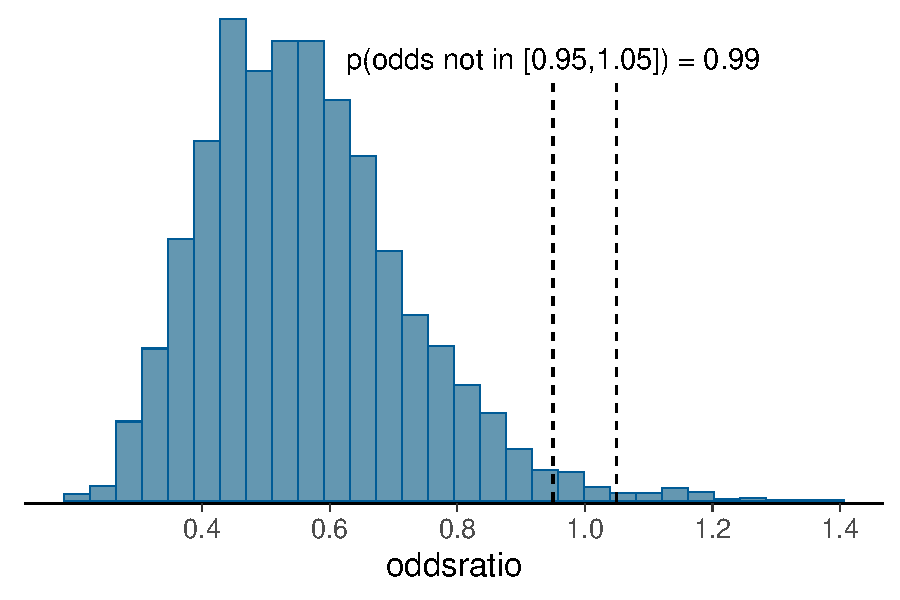
\includegraphics[width=10cm]{odds1_rope.pdf}}
    % \only<2>{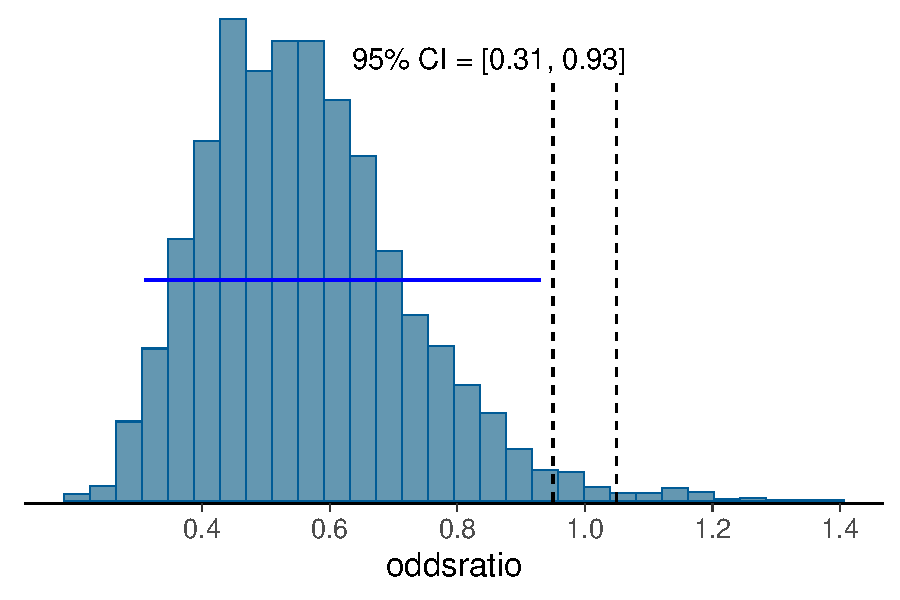
\includegraphics[width=10cm]{odds1_cirope.pdf}}

\end{frame}

\begin{frame}{Bayesian hypothesis testing}

  \begin{itemize}
  \item Instead of hypothesis testing, report full posterior
    \begin{itemize}
      \only<1>{
      \item for continuous posterior there is zero probability that
        e.g. treatment effect is exactly zero
      }
      \only<2>{
      \item for continuous posterior we could compute the probability
        that we know the sign of the effect
      }
      \only<3>{
      \item for continuous posterior some people compare whether
        posterior interval includes null case
      }
      \only<4->{
      \item region of practical equivalence (ROPE)\\
        \phantom{posterior interval includes null case}
      }
    \end{itemize}
  \end{itemize}
  
  \only<1>{\begin{minipage}{14.1cm}
      \hspace{-1.2cm}\includegraphics[width=6.8cm]{odds1_eq.pdf}\includegraphics[width=6.8cm]{odds2_eq.pdf}
    \end{minipage}}
  \only<2>{\begin{minipage}{14.1cm}
      \hspace{-1.2cm}\includegraphics[width=6.8cm]{odds1_less.pdf}\includegraphics[width=6.8cm]{odds2_less.pdf}
    \end{minipage}}
  \only<3>{\begin{minipage}{14.1cm}
      \hspace{-1.2cm}\includegraphics[width=6.8cm]{odds1_ci.pdf}\includegraphics[width=6.8cm]{odds2_ci.pdf}
    \end{minipage}}
  \only<4>{\begin{minipage}{14.1cm}
      \hspace{-1.2cm}\includegraphics[width=6.8cm]{odds1_rope.pdf}\includegraphics[width=6.8cm]{odds2_rope.pdf}
    \end{minipage}}
  % \only<5>{\begin{minipage}{14.1cm}
  %     \hspace{-1.2cm}\includegraphics[width=6.8cm]{odds1_cirope.pdf}\includegraphics[width=6.8cm]{odds2_cirope.pdf}
  %   \end{minipage}}
  
\end{frame}

\begin{frame}{Bayesian hypothesis testing}

  \begin{itemize}
  \item Instead of hypothesis testing, report full posterior
    \begin{itemize}
      \only<1>{
      \item for continuous posterior there is zero probability that
        e.g. treatment effect is exactly zero
      }
      \only<2>{
      \item for continuous posterior we could compute the probability
        that we know the sign of the effect
      }
      \only<3>{
      \item for continuous posterior some people compare whether
        posterior interval includes null case
      }
      \only<4->{
      \item region of practical equivalence (ROPE)\\~
      }
    \end{itemize}
  \end{itemize}
  
  \only<2>{\begin{minipage}{14.1cm}
      \hspace{-1.2cm}\includegraphics[width=6.8cm]{odds2_less.pdf}\includegraphics[width=6.8cm]{odds3_less.pdf}
    \end{minipage}}
  \only<3>{\begin{minipage}{14.1cm}
      \hspace{-1.2cm}\includegraphics[width=6.8cm]{odds2_ci.pdf}\includegraphics[width=6.8cm]{odds3_ci.pdf}
    \end{minipage}}
  \only<4>{\begin{minipage}{14.1cm}
      \hspace{-1.2cm}\includegraphics[width=6.8cm]{odds2_rope.pdf}\includegraphics[width=6.8cm]{odds3_rope.pdf}
    \end{minipage}}
  % \only<5>{\begin{minipage}{14.1cm}
  %     \hspace{-1.2cm}\includegraphics[width=6.8cm]{odds2_cirope.pdf}\includegraphics[width=6.8cm]{odds3_cirope.pdf}
  %   \end{minipage}}
  
\end{frame}

\begin{frame}{Bayesian hypothesis testing}

  \begin{itemize}
  \item Bayes factor
    \begin{itemize}
    \item null model has, e.g., the treatment effect fixed to 0
    \item assumes that there is non-zero probability that the
      treatment effect can be exactly zero (point mass)
    \item requires posterior inference for the null model, too
    \end{itemize}
  \end{itemize}
    \vspace{-1\baselineskip}
  
    \only<1>{\includegraphics[width=9cm]{odds1_bf.pdf}}
    \only<2>{\includegraphics[width=9cm]{odds2_bf.pdf}}
    \only<3>{\includegraphics[width=9cm]{odds3_bf.pdf}}
    \vspace{-1.2\baselineskip}
    
    {\footnotesize\color{gray}\hspace{1cm}  with {\tt bridgesampling} package, see also BDA3 13.10}
\end{frame}

\begin{frame}{Bayesian hypothesis testing}

  \begin{itemize}
  \item Bayes factor
    \begin{itemize}
    \item sensitive to the prior choice even when the posterior is not
    \end{itemize}
  \end{itemize}
  normal(0,3.5) \hspace{4.5cm} normal(0,100)
  \begin{minipage}{14.1cm}
      \hspace{-1.2cm}{\includegraphics[width=6.8cm]{odds1_bf.pdf}}{\includegraphics[width=6.8cm]{odds1_bf100.pdf}}
    \end{minipage}
      \vspace{-1.2\baselineskip}
    {\footnotesize\color{gray}\hspace{1cm}  with {\tt bridgesampling} package, see also BDA3 13.10}
\end{frame}

\begin{frame}[fragile]{Bayesian hypothesis testing}

  \begin{itemize}
  \item Predictive performance
    \begin{itemize}
    \item is there difference in predictive performance with, e.g.,
      treatment effect fixed to zero or unknown treatment effect
    \item requires posterior inference for the null model or
      projection from the full to null
    \item looking at the posterior is better if parameters are
      independent
    \end{itemize}
  \end{itemize}

\end{frame}

\begin{frame}[fragile,fragile]{Bayesian hypothesis testing}

  \begin{itemize}
  \item Predictive performance
    \begin{itemize}
    \item is there difference in predictive performance with, e.g.,
      treatment effect fixed to zero or unknown treatment effect
    \item requires posterior inference for the null model or
      projection from the full to null
    \item looking at the posterior is better if parameters are
      independent
    \end{itemize}
  \end{itemize}

  In the beta blockers example
  \begin{itemize}
  \item Leave-one-person-out works, but is less efficient than looking
    at the posterior (see more in
    \url{https://users.aalto.fi/~ave/modelselection/betablockers.html})
  \end{itemize}

\begin{minted}[fontsize=\footnotesize,escapeinside=\%\%]{r}
> loo_compare(loo(fitb1),loo(fitb2))
      elpd_diff se_diff
fitb2  0.0       0.0   
fitb1 -1.6       2.3   
\end{minted}
  \pause
  \begin{itemize}
  \item For another similar, but more elaborate example, see \url{https://users.aalto.fi/~ave/casestudies/Nabiximols/nabiximols.html}
  \end{itemize}
\end{frame}

% \begin{frame}{Simulation experiment}

%   \vspace{-0.75\baselineskip}
  
%   \begin{minipage}{3.2cm}
%     \vspace{-4\baselineskip}
%     \hfill p(odds < 1)
%   \end{minipage}\includegraphics[width=6cm]{simuridges_beta.pdf}
% \uncover<2->{  
%   \begin{minipage}{3.2cm}
%     \vspace{-4\baselineskip}
%     \hfill Marginal likelihood comparison
%   \end{minipage}\includegraphics[width=6cm]{simuridges_bf.pdf}
%   }
% \uncover<3->{  
%   \vspace{-1\baselineskip}
  
%   \begin{minipage}{3.2cm}
%     \vspace{-4\baselineskip}
%     \hfill LOO comparison
%   \end{minipage}\includegraphics[width=6cm]{simuridges_loo.pdf}
%   \vspace{-1\baselineskip}
%   }
  
% \end{frame}

\begin{frame}{Bodyfat: many predictors}

  \vspace{-0.75\baselineskip}
  \begin{itemize}
  \item Predict bodyfat percentage
  \item The reference value (siri) is obtained by
    immersing person in water. $n=251$.
  \item Which measurements to use in the future?
  \end{itemize}
  \pause
  \vspace{-0.7\baselineskip}
  \includegraphics[width=7cm]{bodyfat_corr.pdf}

\end{frame}

\begin{frame}{Prediction}

  \begin{itemize}
  \item Goal: prediction
  \item<2-> Use all the predictors and sensible prior
    \begin{itemize}
    \item<3-> no model selection needed
    \end{itemize}
  \end{itemize}

\end{frame}

\begin{frame}{Predictive performance based variable selection}

  \begin{itemize}
  \item Goal:
    \begin{itemize}
    \item minimize future measurement cost
    \item easier explainability of the model
    \end{itemize}
  \item<2-> Select the minimal number of covariates with similar
    predictive performance as the full model
  \end{itemize}

\end{frame}

\begin{frame}{Hypothesis testing and posterior dependencies}

  \vspace{-0.5\baselineskip}
  Looking at the marginal posterior $p(\beta < 0)$ can be misleading when there
  are many parameters
  
  Marginal posteriors of coefficients in bodyfat example
  
  \includegraphics[width=10cm]{bodyfat_mcmc_areas.pdf}

\end{frame}

\begin{frame}{Hypothesis testing and posterior dependencies}

  \vspace{-0.75\baselineskip}
  Looking at the marginal posterior(s) can be misleading when there
  are many parameters

  Bivariate marginal of weight and height
  
  \vspace{-0.25\baselineskip}
  \includegraphics[width=6.8cm]{bodyfat_mcmc_scatter.pdf}

\end{frame}

\begin{frame}{Hypothesis testing and posterior dependencies}

  In bodyfat example, starting from full model

  \begin{itemize}
  \item BF in favor of removing weight (p=0.92)
  \item LOO in favor of removing weight (p=0.99)
  \end{itemize}

  In bodyfat example, starting from model y $\sim$ abdomen
  \begin{itemize}
  \item BF in favor of adding weight (p=1.0)
  \item LOO in favor of adding weight (p=1.0)
  \end{itemize}

\end{frame}

\begin{frame}{Predictive performance based variable selection}

  \vspace{-0.75\baselineskip}
  % More elaborate approaches are needed for variable selection
  Projection predictive variable selection selects the minimal set of
  variables with similar predictive performance as the full model
  
  \vspace{-0.5\baselineskip}
  \includegraphics[width=10.5cm]{bodyfat_vsel.pdf}

\end{frame}

\begin{frame}{Projected posterior}

  \vspace{-0.75\baselineskip}
  % More elaborate approaches are needed for variable selection
  Projection predictive variable selection selects the minimal set of
  variables with similar predictive performance as the full model
  
  \includegraphics[width=9cm]{bodyfat_projected.pdf}

  {\footnotesize More about projpred in the end of the course}

\end{frame}

\begin{frame}{Model selection needed to avoid overfitting?}

\begin{list1}
\item Classic example is polynomial model with increasing number of components
  \begin{list2}
  \item overfits also with Bayesian inference and weak priors
  \end{list2}
\end{list1}
\vspace{-0.5\baselineskip}
\only<2>{\includegraphics[height=7cm]{overfit_simdata.pdf}}
\only<3>{\includegraphics[height=7cm]{overfit_elpd_poly.pdf}}

\end{frame}

\begin{frame}{Model selection needed to avoid overfitting?}

\begin{list1}
\item Gaussian process can be used as a prior on function space
  \begin{list2}
  \item GP can be approximated with basis functions
  \item<2-> more basis functions makes the approximation more
    accurate, but doesn't inflate the prior on function space
  \end{list2}
\end{list1}
\vspace{-0.5\baselineskip}

\end{frame}

\begin{frame}{Model is not needed to avoid overfitting}

\begin{list1}
\item Gaussian process can be used as a prior on function space
  \begin{list2}
  \item GP can be approximated with basis functions
  \item more basis functions makes the approximation more
    accurate, but doesn't inflate the prior on function space
  \end{list2}
\end{list1}
\vspace{-0.5\baselineskip}
{\includegraphics[height=6.8cm]{overfit_elpd_GP.pdf}}

\end{frame}

\begin{frame}{Model selection needed to avoid overfitting?}

  logistic regression: 30 \textbf{completely irrelevant} variables, \\100
  observations
  
  \only<2>{\includegraphics[width=10cm]{irrelevant_N.pdf}}

\end{frame}

\begin{frame}{Prior on parameters vs predictions}

N(0,3) prior on each coefficient\\
\only<1>{\includegraphics[width=9cm]{figs/simple.pdf}}
\only<2>{1 variable\\\includegraphics[width=9cm]{prior_N_1.pdf}}
\only<3>{2 variables\\\includegraphics[width=9cm]{prior_N_2.pdf}}
\only<4>{3 variables\\\includegraphics[width=9cm]{prior_N_3.pdf}}
\only<5-6>{30 variables\\\includegraphics[width=9cm]{prior_N_30.pdf}}

\only<6>{A weak prior on parameters can be a strong prior on
  predictions that favors overfitting}

\end{frame}

\begin{frame}{Better priors}

N(0,$\frac{1}{\sqrt{p}}$) prior on each coefficient\\
\only<1>{\includegraphics[width=9cm]{figs/simple.pdf}}
\only<2>{1 variable\\\includegraphics[width=9cm]{prior_Ns_1.pdf}}
\only<3>{2 variables\\\includegraphics[width=9cm]{prior_Ns_2.pdf}}
\only<4>{3 variables\\\includegraphics[width=9cm]{prior_Ns_3.pdf}}
\only<5-6>{30 variables\\\includegraphics[width=9cm]{prior_Ns_30.pdf}}

\only<6>{Prior on predictions (almost) fixed when the model gets bigger}
  
\end{frame}

\begin{frame}{Better priors, no overfitting}

  logistic regression: 30 \textbf{completely irrelevant} variables, \\100
  observations,
  \only<1>{N(0,$\frac{1}{\sqrt{p}}$) prior}
  \only<2>{regularized horseshoe prior}
  
  \only<1>{\includegraphics[width=10cm]{irrelevant_Ns.pdf}}
  \only<2>{\includegraphics[width=10cm]{irrelevant_RHS.pdf}}
  
\end{frame}

\begin{frame}{Many weak effects, wide prior on parameters}

  logistic regression: 30 \textbf{weakly relevant} variables, \\100
  observations, N(0,3) prior
  
  {\includegraphics[width=10cm]{weak_N.pdf}}

\end{frame}

\begin{frame}{Many weak effects, better prior}

  logistic regression: 30 \textbf{weakly relevant} variables, \\100
  observations, N(0,$\frac{1}{\sqrt{p}}$) prior
  
  {\includegraphics[width=10cm]{weak_Ns.pdf}}

\end{frame}

\begin{frame}{Correlating variables, wide prior on parameters}

  logistic regression: 30 \textbf{correlating relevant} variables, \\100
  observations, N(0,3) prior
  
  % \only<1>{\includegraphics[width=9cm]{figs/simple.pdf}}
  {\includegraphics[width=10cm]{correlating_N.pdf}}

\end{frame}

\begin{frame}{Correlating variables, better prior}

  logistic regression: 30 \textbf{correlating relevant} variables, \\100
  observations
  {N(0,$\frac{1}{\sqrt{p}}$) prior}
  
  {\includegraphics[width=10cm]{correlating_Ns.pdf}}

\end{frame}

\begin{frame}{Implied prior on $R^2$}

  Regression and Other Stories, Section 12.7 Models for regression
  coefficients: 

  \only<1>{Wide prior on coefficients favors overfitting\\\includegraphics[width=6cm]{student_fit1_R2.pdf}}
  \only<2>{Scaled prior on coefficients\\\includegraphics[width=6cm]{student_fit2_R2.pdf}}
  \only<3>{Regularized horseshoe prior on coefficients\\\includegraphics[width=6cm]{student_fit3_R2.pdf}}

  
\end{frame}

\begin{frame}{Better priors}

  For example:
  \begin{itemize}
  \item scaled: many weak effects
  \item regularized horseshoe, R2-D2: only some relevant
  \item R2-D2: defined directly for $R^2$
  \item PCA-type: highly correlating variables
  \end{itemize}

\end{frame}


\begin{frame}{$p \gg n$}

  \begin{itemize}
  \item With good priors, possible to have more variables than observations
  \item e.g. $p=22283, n=85$ demonstrated by Piironen, Paasiniemi,
    Vehtari (2020)
  \end{itemize}
\end{frame}


\begin{frame}{Variable selection}
  
  Variable selection
  \begin{itemize}
  \item[1.] is not needed to avoid overfitting
  \item[2.] can be used to reduce costs and improve explainability
  \end{itemize}

\end{frame}

% \begin{frame}{Model selection is not needed to avoid overfitting}

% \begin{list1}
% \item No overfitting when using good priors that keep the prior on the
%   predictive space approximately constant when more components are
%   added, e.g.
%   \begin{list2}
%     \item Gaussian processes
%     \item (regularized) Horseshoe for sparsity
%     \item R2-D2 and R2-D2-M2 for prior on $R^2$
%   \end{list2}
% \end{list1}

% \end{frame}

\begin{frame}{Model selection can overfit}

  \begin{list1}
  \item Selection induced bias in cross-validation
    \begin{list2}
    \item same data is used to assess the performance and make the selection
    \item the selected model fits more to the data
    \item the CV estimate for the selected model is biased
    \item recognized already, e.g., by Stone (1974)
    \end{list2}
    \pause
  \item Performance of the selection process itself can be assessed
    using two level cross-validation, but it does not help choosing
    better models
    \pause
  \item Bigger problem if there is a large number of models as in
    covariate selection
  \end{list1}

\end{frame}

\begin{frame}{Model selection can overfit}

  \begin{itemize}
  \item Variable selection with forward selection
    \begin{itemize}
    \item start with null model
    \item add the variable improving the predictive performance most
    \item add the next variable improving... and so on
    \end{itemize}
  \end{itemize}

  \only<2>{\includegraphics[width=10cm]{overfit.pdf}}
  
\end{frame}

\begin{frame}{Model selection can overfit}

  \vspace{-0.7\baselineskip}
  \only<1>{Wide normal prior\\
    \includegraphics[width=10.5cm]{gaussian_forward.pdf}}
  \only<2->{R2D2 prior reduces overfit in model selection\\
    \includegraphics[width=10.5cm]{r2d2_forward.pdf}\\}

  \vspace{-\baselineskip}
  \uncover<3>{Reminder: variable selection is not needed with good priors
    to get good predictive performance, but may be useful for other purposes}

\end{frame}

% \begin{frame}{Selection induced bias in variable selection}

%   \includegraphics[width=\textwidth]{cv.pdf}

% \end{frame}

% \begin{frame}{Selection induced bias in variable selection}

%   \includegraphics[height=0.88\textheight]{simulated_searchpath.pdf}
%    \vspace{-1.5\baselineskip}
%    \mbox{{\hspace{8cm} \footnotesize \href{http://link.springer.com/article/10.1007/s11222-016-9649-y}{Piironen \& Vehtari (2017)}}}

% \end{frame}

% \begin{frame}{What if one is not clearly better than others?}

%   \begin{list1}
%   \item<2-> Continuous expansion including all models?
%     \begin{list2}
%     \item and then analyse the posterior distribution directly
%     \item sparse priors like R2D2 prior instead of variable selection
%     \end{list2}
%   \item<3-> Model averaging with BMA or Bayesian stacking?
%   \item<4-> In a nested case choose simpler if assuming some cost for
%     extra parts?
%   \item<5-> In a nested case choose more complex if you want to take
%     into account all the uncertainties.
%   \end{list1}

% \end{frame}

\begin{frame}{Model averaging}
  
  \begin{list1}
  \item<+-> Prefer continuous model expansion
  \item<+-> If needed integrate over the model space = model averaging
  \item<+-> Bayesian model averaging is just the usual integration
    over unknowns
  \item<+-> Bayesian stacking may work better than BMA in case of
    misspecified models or small data
    \begin{list2}
    \item \href{https://projecteuclid.org/euclid.ba/1516093227}{Yao, Vehtari, Simpson, and Gelman (2018). Using stacking to average Bayesian predictive distributions (with discussion). \textit{Bayesian Analysis}, 13(3):917-1003}
    \end{list2}
  \end{list1}
  
\end{frame}

\begin{frame}{ Cross-validation and model selection}

  \begin{list1}
  \item<1-> Cross-validation can be used for model selection if
    \begin{list2}
      \item small number of models
      \item the difference between models is clear
    \end{list2}
  \item<2-> Be careful if using cross-validation to choose from a large set of models
    \begin{list2}
    \item selection process can lead to severe overfitting
    % \item you may use projection predictive approach
    % \item useful when correlating variables make the posterior
    %   distribution analysis difficult\\
    %   {\small video, refs and demos  at \url{avehtari.github.io/modelselection/}\\
    %   and \href{http://link.springer.com/article/10.1007/s11222-016-9649-y}{Piironen \& Vehtari (2017)}}
    \end{list2}
  \item<3-> Overfitting in selection process is not unique for cross-validation
  \end{list1}
\end{frame}

% \begin{frame}

%   {\Large\color{navyblue} Selection induced bias in variable selection}

%   \includegraphics[height=0.88\textheight]{simulated_variability.pdf}
%    \vspace{-1.5\baselineskip}
%    \mbox{{\hspace{8cm} \footnotesize \href{http://link.springer.com/article/10.1007/s11222-016-9649-y}{Piironen \& Vehtari (2017)}}}

% \end{frame}

% \begin{frame}

%   {\Large\color{navyblue} Selection induced bias in variable selection}

%   \includegraphics[height=0.88\textheight]{real_searchpath.pdf}
%    \vspace{-2\baselineskip}
%    \mbox{{\hspace{9.5cm} \parbox[t]{12cm}{\footnotesize \href{http://link.springer.com/article/10.1007/s11222-016-9649-y}{Piironen \&\\ Vehtari (2017)}}}}

% \end{frame}

\begin{frame}{Take-home messages}

  \begin{list1}
  \item It's good to think predictions of observables, because
    observables are the only ones we can observe
  \item \only<1>{\color{gray}}Cross-validation can simulate predicting and observing new
    data
  \item \only<2>{\color{gray}}Cross-validation is good if you don't
    trust your model
  \item \only<3>{\color{gray}}Different variants of cross-validation
    are useful in different scenarios
  \item \only<4>{\color{gray}}Cross-validation has high variance, and
    {\bf if} you trust your model you can beat cross-validation in
    accuracy
  \end{list1}
  \only<5>{~}

\end{frame}

\end{document}

%%% Local Variables: 
%%% mode: latex
%%% TeX-master: t
%%% TeX-command-extra-options: "-shell-escape"
%%% End:
